% das hier ist gerade nur eine Kopie von den l2 slides


\documentclass[11pt,compress,t,notes=noshow, xcolor=table]{beamer}
\documentclass[11pt,compress,t,notes=noshow, xcolor=table]{beamer}
\usepackage[]{graphicx}\usepackage[]{color}
% maxwidth is the original width if it is less than linewidth
% otherwise use linewidth (to make sure the graphics do not exceed the margin)
\makeatletter
\def\maxwidth{ %
  \ifdim\Gin@nat@width>\linewidth
    \linewidth
  \else
    \Gin@nat@width
  \fi
}
\makeatother

\definecolor{fgcolor}{rgb}{0.345, 0.345, 0.345}
\newcommand{\hlnum}[1]{\textcolor[rgb]{0.686,0.059,0.569}{#1}}%
\newcommand{\hlstr}[1]{\textcolor[rgb]{0.192,0.494,0.8}{#1}}%
\newcommand{\hlcom}[1]{\textcolor[rgb]{0.678,0.584,0.686}{\textit{#1}}}%
\newcommand{\hlopt}[1]{\textcolor[rgb]{0,0,0}{#1}}%
\newcommand{\hlstd}[1]{\textcolor[rgb]{0.345,0.345,0.345}{#1}}%
\newcommand{\hlkwa}[1]{\textcolor[rgb]{0.161,0.373,0.58}{\textbf{#1}}}%
\newcommand{\hlkwb}[1]{\textcolor[rgb]{0.69,0.353,0.396}{#1}}%
\newcommand{\hlkwc}[1]{\textcolor[rgb]{0.333,0.667,0.333}{#1}}%
\newcommand{\hlkwd}[1]{\textcolor[rgb]{0.737,0.353,0.396}{\textbf{#1}}}%
\let\hlipl\hlkwb

\usepackage{framed}
\makeatletter
\newenvironment{kframe}{%
 \def\at@end@of@kframe{}%
 \ifinner\ifhmode%
  \def\at@end@of@kframe{\end{minipage}}%
  \begin{minipage}{\columnwidth}%
 \fi\fi%
 \def\FrameCommand##1{\hskip\@totalleftmargin \hskip-\fboxsep
 \colorbox{shadecolor}{##1}\hskip-\fboxsep
     % There is no \\@totalrightmargin, so:
     \hskip-\linewidth \hskip-\@totalleftmargin \hskip\columnwidth}%
 \MakeFramed {\advance\hsize-\width
   \@totalleftmargin\z@ \linewidth\hsize
   \@setminipage}}%
 {\par\unskip\endMakeFramed%
 \at@end@of@kframe}
\makeatother

\definecolor{shadecolor}{rgb}{.97, .97, .97}
\definecolor{messagecolor}{rgb}{0, 0, 0}
\definecolor{warningcolor}{rgb}{1, 0, 1}
\definecolor{errorcolor}{rgb}{1, 0, 0}
\newenvironment{knitrout}{}{} % an empty environment to be redefined in TeX

\usepackage{alltt}
\newcommand{\SweaveOpts}[1]{}  % do not interfere with LaTeX
\newcommand{\SweaveInput}[1]{} % because they are not real TeX commands
\newcommand{\Sexpr}[1]{}       % will only be parsed by R
\newcommand{\xmark}{\ding{55}}%


\usepackage[english]{babel}
\usepackage[utf8]{inputenc}

\usepackage{dsfont}
\usepackage{verbatim}
\usepackage{amsmath}
\usepackage{amsfonts}
\usepackage{amssymb}
\usepackage{bm}
\usepackage{csquotes}
\usepackage{multirow}
\usepackage{longtable}
\usepackage{booktabs}
\usepackage{enumerate}
\usepackage[absolute,overlay]{textpos}
\usepackage{psfrag}
\usepackage{algorithm}
\usepackage{algpseudocode}
\usepackage{eqnarray}
\usepackage{arydshln}
\usepackage{tabularx}
\usepackage{placeins}
\usepackage{tikz}
\usepackage{setspace}
\usepackage{colortbl}
\usepackage{mathtools}
\usepackage{wrapfig}
\usepackage{bm}
\usepackage{amsmath}
\usepackage{pifont}

\usetikzlibrary{shapes,arrows,automata,positioning,calc,chains,trees, shadows}
\tikzset{
  %Define standard arrow tip
  >=stealth',
  %Define style for boxes
  punkt/.style={
    rectangle,
    rounded corners,
    draw=black, very thick,
    text width=6.5em,
    minimum height=2em,
    text centered},
  % Define arrow style
  pil/.style={
    ->,
    thick,
    shorten <=2pt,
    shorten >=2pt,}
}

\usepackage{subfig}

% Defines macros and environments
\usepackage{../../style/lmu-lecture}


\let\code=\texttt
\let\proglang=\textsf

\setkeys{Gin}{width=0.9\textwidth}

\setbeamertemplate{frametitle}{\expandafter\uppercase\expandafter\insertframetitle}

\usepackage{bbm}
% basic latex stuff
\newcommand{\pkg}[1]{{\fontseries{b}\selectfont #1}} %fontstyle for R packages
\newcommand{\lz}{\vspace{0.5cm}} %vertical space
\newcommand{\dlz}{\vspace{1cm}} %double vertical space
\newcommand{\oneliner}[1] % Oneliner for important statements
{\begin{block}{}\begin{center}\begin{Large}#1\end{Large}\end{center}\end{block}}


%new environments
\newenvironment{vbframe}  %frame with breaks and verbatim
{
 \begin{frame}[containsverbatim,allowframebreaks]
}
{
\end{frame}
}

\newenvironment{vframe}  %frame with verbatim without breaks (to avoid numbering one slided frames)
{
 \begin{frame}[containsverbatim]
}
{
\end{frame}
}

\newenvironment{blocki}[1]   % itemize block
{
 \begin{block}{#1}\begin{itemize}
}
{
\end{itemize}\end{block}
}

\newenvironment{fragileframe}[2]{  %fragile frame with framebreaks
\begin{frame}[allowframebreaks, fragile, environment = fragileframe]
\frametitle{#1}
#2}
{\end{frame}}


\newcommand{\myframe}[2]{  %short for frame with framebreaks
\begin{frame}[allowframebreaks]
\frametitle{#1}
#2
\end{frame}}

\newcommand{\remark}[1]{
  \textbf{Remark:} #1
}

\newcommand{\citebutton}[2]{%
\NoCaseChange{\resizebox{!}{9pt}{\protect\beamergotobutton{\href{#2}{#1}}}}%
}



\newenvironment{deleteframe}
{
\begingroup
\usebackgroundtemplate{\includegraphics[width=\paperwidth,height=\paperheight]{../style/color/red.png}}
 \begin{frame}
}
{
\end{frame}
\endgroup
}
\newenvironment{simplifyframe}
{
\begingroup
\usebackgroundtemplate{\includegraphics[width=\paperwidth,height=\paperheight]{../style/color/yellow.png}}
 \begin{frame}
}
{
\end{frame}
\endgroup
}\newenvironment{draftframe}
{
\begingroup
\usebackgroundtemplate{\includegraphics[width=\paperwidth,height=\paperheight]{../style/color/green.jpg}}
 \begin{frame}
}
{
\end{frame}
\endgroup
}
% https://tex.stackexchange.com/a/261480: textcolor that works in mathmode
\makeatletter
\renewcommand*{\@textcolor}[3]{%
  \protect\leavevmode
  \begingroup
    \color#1{#2}#3%
  \endgroup
}
\makeatother





% math spaces
\ifdefined\N                                                                
\renewcommand{\N}{\mathds{N}} % N, naturals
\else \newcommand{\N}{\mathds{N}} \fi 
\newcommand{\Z}{\mathds{Z}} % Z, integers
\newcommand{\Q}{\mathds{Q}} % Q, rationals
\newcommand{\R}{\mathds{R}} % R, reals
\ifdefined\C 
  \renewcommand{\C}{\mathds{C}} % C, complex
\else \newcommand{\C}{\mathds{C}} \fi
\newcommand{\continuous}{\mathcal{C}} % C, space of continuous functions
\newcommand{\M}{\mathcal{M}} % machine numbers
\newcommand{\epsm}{\epsilon_m} % maximum error

% counting / finite sets
\newcommand{\setzo}{\{0, 1\}} % set 0, 1
\newcommand{\setmp}{\{-1, +1\}} % set -1, 1
\newcommand{\unitint}{[0, 1]} % unit interval

% basic math stuff
\newcommand{\xt}{\tilde x} % x tilde
\newcommand{\argmax}{\operatorname{arg\,max}} % argmax
\newcommand{\argmin}{\operatorname{arg\,min}} % argmin
\newcommand{\argminlim}{\mathop{\mathrm{arg\,min}}\limits} % argmax with limits
\newcommand{\argmaxlim}{\mathop{\mathrm{arg\,max}}\limits} % argmin with limits  
\newcommand{\sign}{\operatorname{sign}} % sign, signum
\newcommand{\I}{\mathbb{I}} % I, indicator
\newcommand{\order}{\mathcal{O}} % O, order
\newcommand{\pd}[2]{\frac{\partial{#1}}{\partial #2}} % partial derivative
\newcommand{\floorlr}[1]{\left\lfloor #1 \right\rfloor} % floor
\newcommand{\ceillr}[1]{\left\lceil #1 \right\rceil} % ceiling

% sums and products
\newcommand{\sumin}{\sum\limits_{i=1}^n} % summation from i=1 to n
\newcommand{\sumim}{\sum\limits_{i=1}^m} % summation from i=1 to m
\newcommand{\sumjn}{\sum\limits_{j=1}^n} % summation from j=1 to p
\newcommand{\sumjp}{\sum\limits_{j=1}^p} % summation from j=1 to p
\newcommand{\sumik}{\sum\limits_{i=1}^k} % summation from i=1 to k
\newcommand{\sumkg}{\sum\limits_{k=1}^g} % summation from k=1 to g
\newcommand{\sumjg}{\sum\limits_{j=1}^g} % summation from j=1 to g
\newcommand{\meanin}{\frac{1}{n} \sum\limits_{i=1}^n} % mean from i=1 to n
\newcommand{\meanim}{\frac{1}{m} \sum\limits_{i=1}^m} % mean from i=1 to n
\newcommand{\meankg}{\frac{1}{g} \sum\limits_{k=1}^g} % mean from k=1 to g
\newcommand{\prodin}{\prod\limits_{i=1}^n} % product from i=1 to n
\newcommand{\prodkg}{\prod\limits_{k=1}^g} % product from k=1 to g
\newcommand{\prodjp}{\prod\limits_{j=1}^p} % product from j=1 to p

% linear algebra
\newcommand{\one}{\boldsymbol{1}} % 1, unitvector
\newcommand{\zero}{\mathbf{0}} % 0-vector
\newcommand{\id}{\boldsymbol{I}} % I, identity
\newcommand{\diag}{\operatorname{diag}} % diag, diagonal
\newcommand{\trace}{\operatorname{tr}} % tr, trace
\newcommand{\spn}{\operatorname{span}} % span
\newcommand{\scp}[2]{\left\langle #1, #2 \right\rangle} % <.,.>, scalarproduct
\newcommand{\mat}[1]{\begin{pmatrix} #1 \end{pmatrix}} % short pmatrix command
\newcommand{\Amat}{\mathbf{A}} % matrix A
\newcommand{\Deltab}{\mathbf{\Delta}} % error term for vectors

% basic probability + stats
\renewcommand{\P}{\mathds{P}} % P, probability
\newcommand{\E}{\mathds{E}} % E, expectation
\newcommand{\var}{\mathsf{Var}} % Var, variance
\newcommand{\cov}{\mathsf{Cov}} % Cov, covariance
\newcommand{\corr}{\mathsf{Corr}} % Corr, correlation
\newcommand{\normal}{\mathcal{N}} % N of the normal distribution
\newcommand{\iid}{\overset{i.i.d}{\sim}} % dist with i.i.d superscript
\newcommand{\distas}[1]{\overset{#1}{\sim}} % ... is distributed as ...

% machine learning
\newcommand{\Xspace}{\mathcal{X}} % X, input space
\newcommand{\Yspace}{\mathcal{Y}} % Y, output space
\newcommand{\nset}{\{1, \ldots, n\}} % set from 1 to n
\newcommand{\pset}{\{1, \ldots, p\}} % set from 1 to p
\newcommand{\gset}{\{1, \ldots, g\}} % set from 1 to g
\newcommand{\Pxy}{\mathbb{P}_{xy}} % P_xy
\newcommand{\Exy}{\mathbb{E}_{xy}} % E_xy: Expectation over random variables xy
\newcommand{\xv}{\mathbf{x}} % vector x (bold)
\newcommand{\xtil}{\tilde{\mathbf{x}}} % vector x-tilde (bold)
\newcommand{\yv}{\mathbf{y}} % vector y (bold)
\newcommand{\xy}{(\xv, y)} % observation (x, y)
\newcommand{\xvec}{\left(x_1, \ldots, x_p\right)^\top} % (x1, ..., xp) 
\newcommand{\Xmat}{\mathbf{X}} % Design matrix
\newcommand{\allDatasets}{\mathds{D}} % The set of all datasets
\newcommand{\allDatasetsn}{\mathds{D}_n}  % The set of all datasets of size n 
\newcommand{\D}{\mathcal{D}} % D, data
\newcommand{\Dn}{\D_n} % D_n, data of size n
\newcommand{\Dtrain}{\mathcal{D}_{\text{train}}} % D_train, training set
\newcommand{\Dtest}{\mathcal{D}_{\text{test}}} % D_test, test set
\newcommand{\xyi}[1][i]{\left(\xv^{(#1)}, y^{(#1)}\right)} % (x^i, y^i), i-th observation
\newcommand{\Dset}{\left( \xyi[1], \ldots, \xyi[n]\right)} % {(x1,y1)), ..., (xn,yn)}, data
\newcommand{\defAllDatasetsn}{(\Xspace \times \Yspace)^n} % Def. of the set of all datasets of size n 
\newcommand{\defAllDatasets}{\bigcup_{n \in \N}(\Xspace \times \Yspace)^n} % Def. of the set of all datasets 
\newcommand{\xdat}{\left\{ \xv^{(1)}, \ldots, \xv^{(n)}\right\}} % {x1, ..., xn}, input data
\newcommand{\yvec}{\left(y^{(1)}, \hdots, y^{(n)}\right)^\top} % (y1, ..., yn), vector of outcomes
\renewcommand{\xi}[1][i]{\xv^{(#1)}} % x^i, i-th observed value of x
\newcommand{\yi}[1][i]{y^{(#1)}} % y^i, i-th observed value of y 
\newcommand{\xivec}{\left(x^{(i)}_1, \ldots, x^{(i)}_p\right)^\top} % (x1^i, ..., xp^i), i-th observation vector
\newcommand{\xj}{\xv_j} % x_j, j-th feature
\newcommand{\xjvec}{\left(x^{(1)}_j, \ldots, x^{(n)}_j\right)^\top} % (x^1_j, ..., x^n_j), j-th feature vector
\newcommand{\phiv}{\mathbf{\phi}} % Basis transformation function phi
\newcommand{\phixi}{\mathbf{\phi}^{(i)}} % Basis transformation of xi: phi^i := phi(xi)

%%%%%% ml - models general
\newcommand{\lamv}{\bm{\lambda}} % lambda vector, hyperconfiguration vector
\newcommand{\Lam}{\bm{\Lambda}}	 % Lambda, space of all hpos
% Inducer / Inducing algorithm
\newcommand{\preimageInducer}{\left(\defAllDatasets\right)\times\Lam} % Set of all datasets times the hyperparameter space
\newcommand{\preimageInducerShort}{\allDatasets\times\Lam} % Set of all datasets times the hyperparameter space
% Inducer / Inducing algorithm
\newcommand{\ind}{\mathcal{I}} % Inducer, inducing algorithm, learning algorithm 

% continuous prediction function f
\newcommand{\ftrue}{f_{\text{true}}}  % True underlying function (if a statistical model is assumed)
\newcommand{\ftruex}{\ftrue(\xv)} % True underlying function (if a statistical model is assumed)
\newcommand{\fx}{f(\xv)} % f(x), continuous prediction function
\newcommand{\fdomains}{f: \Xspace \rightarrow \R^g} % f with domain and co-domain
\newcommand{\Hspace}{\mathcal{H}} % hypothesis space where f is from
\newcommand{\fbayes}{f^{\ast}} % Bayes-optimal model
\newcommand{\fxbayes}{f^{\ast}(\xv)} % Bayes-optimal model
\newcommand{\fkx}[1][k]{f_{#1}(\xv)} % f_j(x), discriminant component function
\newcommand{\fh}{\hat{f}} % f hat, estimated prediction function
\newcommand{\fxh}{\fh(\xv)} % fhat(x)
\newcommand{\fxt}{f(\xv ~|~ \thetab)} % f(x | theta)
\newcommand{\fxi}{f\left(\xv^{(i)}\right)} % f(x^(i))
\newcommand{\fxih}{\hat{f}\left(\xv^{(i)}\right)} % f(x^(i))
\newcommand{\fxit}{f\left(\xv^{(i)} ~|~ \thetab\right)} % f(x^(i) | theta)
\newcommand{\fhD}{\fh_{\D}} % fhat_D, estimate of f based on D
\newcommand{\fhDtrain}{\fh_{\Dtrain}} % fhat_Dtrain, estimate of f based on D
\newcommand{\fhDnlam}{\fh_{\Dn, \lamv}} %model learned on Dn with hp lambda
\newcommand{\fhDlam}{\fh_{\D, \lamv}} %model learned on D with hp lambda
\newcommand{\fhDnlams}{\fh_{\Dn, \lamv^\ast}} %model learned on Dn with optimal hp lambda 
\newcommand{\fhDlams}{\fh_{\D, \lamv^\ast}} %model learned on D with optimal hp lambda 

% discrete prediction function h
\newcommand{\hx}{h(\xv)} % h(x), discrete prediction function
\newcommand{\hh}{\hat{h}} % h hat
\newcommand{\hxh}{\hat{h}(\xv)} % hhat(x)
\newcommand{\hxt}{h(\xv | \thetab)} % h(x | theta)
\newcommand{\hxi}{h\left(\xi\right)} % h(x^(i))
\newcommand{\hxit}{h\left(\xi ~|~ \thetab\right)} % h(x^(i) | theta)
\newcommand{\hbayes}{h^{\ast}} % Bayes-optimal classification model
\newcommand{\hxbayes}{h^{\ast}(\xv)} % Bayes-optimal classification model

% yhat
\newcommand{\yh}{\hat{y}} % yhat for prediction of target
\newcommand{\yih}{\hat{y}^{(i)}} % yhat^(i) for prediction of ith targiet
\newcommand{\resi}{\yi- \yih}

% theta
\newcommand{\thetah}{\hat{\theta}} % theta hat
\newcommand{\thetab}{\bm{\theta}} % theta vector
\newcommand{\thetabh}{\bm{\hat\theta}} % theta vector hat
\newcommand{\thetat}[1][t]{\thetab^{[#1]}} % theta^[t] in optimization
\newcommand{\thetatn}[1][t]{\thetab^{[#1 +1]}} % theta^[t+1] in optimization
\newcommand{\thetahDnlam}{\thetabh_{\Dn, \lamv}} %theta learned on Dn with hp lambda
\newcommand{\thetahDlam}{\thetabh_{\D, \lamv}} %theta learned on D with hp lambda
\newcommand{\mint}{\min_{\thetab \in \Theta}} % min problem theta
\newcommand{\argmint}{\argmin_{\thetab \in \Theta}} % argmin theta

% densities + probabilities
% pdf of x 
\newcommand{\pdf}{p} % p
\newcommand{\pdfx}{p(\xv)} % p(x)
\newcommand{\pixt}{\pi(\xv~|~ \thetab)} % pi(x|theta), pdf of x given theta
\newcommand{\pixit}{\pi\left(\xi ~|~ \thetab\right)} % pi(x^i|theta), pdf of x given theta
\newcommand{\pixii}{\pi\left(\xi\right)} % pi(x^i), pdf of i-th x 

% pdf of (x, y)
\newcommand{\pdfxy}{p(\xv,y)} % p(x, y)
\newcommand{\pdfxyt}{p(\xv, y ~|~ \thetab)} % p(x, y | theta)
\newcommand{\pdfxyit}{p\left(\xi, \yi ~|~ \thetab\right)} % p(x^(i), y^(i) | theta)

% pdf of x given y
\newcommand{\pdfxyk}[1][k]{p(\xv | y= #1)} % p(x | y = k)
\newcommand{\lpdfxyk}[1][k]{\log p(\xv | y= #1)} % log p(x | y = k)
\newcommand{\pdfxiyk}[1][k]{p\left(\xi | y= #1 \right)} % p(x^i | y = k)

% prior probabilities
\newcommand{\pik}[1][k]{\pi_{#1}} % pi_k, prior
\newcommand{\lpik}[1][k]{\log \pi_{#1}} % log pi_k, log of the prior
\newcommand{\pit}{\pi(\thetab)} % Prior probability of parameter theta

% posterior probabilities
\newcommand{\post}{\P(y = 1 ~|~ \xv)} % P(y = 1 | x), post. prob for y=1
\newcommand{\postk}[1][k]{\P(y = #1 ~|~ \xv)} % P(y = k | y), post. prob for y=k
\newcommand{\pidomains}{\pi: \Xspace \rightarrow \unitint} % pi with domain and co-domain
\newcommand{\pibayes}{\pi^{\ast}} % Bayes-optimal classification model
\newcommand{\pixbayes}{\pi^{\ast}(\xv)} % Bayes-optimal classification model
\newcommand{\pix}{\pi(\xv)} % pi(x), P(y = 1 | x)
\newcommand{\pikx}[1][k]{\pi_{#1}(\xv)} % pi_k(x), P(y = k | x)
\newcommand{\pikxt}[1][k]{\pi_{#1}(\xv ~|~ \thetab)} % pi_k(x | theta), P(y = k | x, theta)
\newcommand{\pixh}{\hat \pi(\xv)} % pi(x) hat, P(y = 1 | x) hat
\newcommand{\pikxh}[1][k]{\hat \pi_{#1}(\xv)} % pi_k(x) hat, P(y = k | x) hat
\newcommand{\pixih}{\hat \pi(\xi)} % pi(x^(i)) with hat
\newcommand{\pikxih}[1][k]{\hat \pi_{#1}(\xi)} % pi_k(x^(i)) with hat
\newcommand{\pdfygxt}{p(y ~|~\xv, \thetab)} % p(y | x, theta)
\newcommand{\pdfyigxit}{p\left(\yi ~|~\xi, \thetab\right)} % p(y^i |x^i, theta)
\newcommand{\lpdfygxt}{\log \pdfygxt } % log p(y | x, theta)
\newcommand{\lpdfyigxit}{\log \pdfyigxit} % log p(y^i |x^i, theta)

% probababilistic
\newcommand{\bayesrulek}[1][k]{\frac{\P(\xv | y= #1) \P(y= #1)}{\P(\xv)}} % Bayes rule
\newcommand{\muk}{\bm{\mu_k}} % mean vector of class-k Gaussian (discr analysis) 

% residual and margin
\newcommand{\eps}{\epsilon} % residual, stochastic
\newcommand{\epsi}{\epsilon^{(i)}} % epsilon^i, residual, stochastic
\newcommand{\epsh}{\hat{\epsilon}} % residual, estimated
\newcommand{\yf}{y \fx} % y f(x), margin
\newcommand{\yfi}{\yi \fxi} % y^i f(x^i), margin
\newcommand{\Sigmah}{\hat \Sigma} % estimated covariance matrix
\newcommand{\Sigmahj}{\hat \Sigma_j} % estimated covariance matrix for the j-th class

% ml - loss, risk, likelihood
\newcommand{\Lyf}{L\left(y, f\right)} % L(y, f), loss function
\newcommand{\Lxy}{L\left(y, \fx\right)} % L(y, f(x)), loss function
\newcommand{\Lxyi}{L\left(\yi, \fxi\right)} % loss of observation
\newcommand{\Lxyt}{L\left(y, \fxt\right)} % loss with f parameterized
\newcommand{\Lxyit}{L\left(\yi, \fxit\right)} % loss of observation with f parameterized
\newcommand{\Lxym}{L\left(\yi, f\left(\bm{\tilde{x}}^{(i)} ~|~ \thetab\right)\right)} % loss of observation with f parameterized
\newcommand{\Lpixy}{L\left(y, \pix\right)} % loss in classification
\newcommand{\Lpixyi}{L\left(\yi, \pixii\right)} % loss of observation in classification
\newcommand{\Lpixyt}{L\left(y, \pixt\right)} % loss with pi parameterized
\newcommand{\Lpixyit}{L\left(\yi, \pixit\right)} % loss of observation with pi parameterized
\newcommand{\Lhxy}{L\left(y, \hx\right)} % L(y, h(x)), loss function on discrete classes
\newcommand{\Lr}{L\left(r\right)} % L(r), loss defined on residual (reg) / margin (classif)
\newcommand{\lone}{|y - \fx|} % L1 loss
\newcommand{\ltwo}{\left(y - \fx\right)^2} % L2 loss
\newcommand{\lbernoullimp}{\ln(1 + \exp(-y \cdot \fx))} % Bernoulli loss for -1, +1 encoding
\newcommand{\lbernoullizo}{- y \cdot \fx + \log(1 + \exp(\fx))} % Bernoulli loss for 0, 1 encoding
\newcommand{\lcrossent}{- y \log \left(\pix\right) - (1 - y) \log \left(1 - \pix\right)} % cross-entropy loss
\newcommand{\lbrier}{\left(\pix - y \right)^2} % Brier score
\newcommand{\risk}{\mathcal{R}} % R, risk
\newcommand{\riskbayes}{\mathcal{R}^\ast}
\newcommand{\riskf}{\risk(f)} % R(f), risk
\newcommand{\riskdef}{\E_{y|\xv}\left(\Lxy \right)} % risk def (expected loss)
\newcommand{\riskt}{\mathcal{R}(\thetab)} % R(theta), risk
\newcommand{\riske}{\mathcal{R}_{\text{emp}}} % R_emp, empirical risk w/o factor 1 / n
\newcommand{\riskeb}{\bar{\mathcal{R}}_{\text{emp}}} % R_emp, empirical risk w/ factor 1 / n
\newcommand{\riskef}{\riske(f)} % R_emp(f)
\newcommand{\risket}{\mathcal{R}_{\text{emp}}(\thetab)} % R_emp(theta)
\newcommand{\riskr}{\mathcal{R}_{\text{reg}}} % R_reg, regularized risk
\newcommand{\riskrt}{\mathcal{R}_{\text{reg}}(\thetab)} % R_reg(theta)
\newcommand{\riskrf}{\riskr(f)} % R_reg(f)
\newcommand{\riskrth}{\hat{\mathcal{R}}_{\text{reg}}(\thetab)} % hat R_reg(theta)
\newcommand{\risketh}{\hat{\mathcal{R}}_{\text{emp}}(\thetab)} % hat R_emp(theta)
\newcommand{\LL}{\mathcal{L}} % L, likelihood
\newcommand{\LLt}{\mathcal{L}(\thetab)} % L(theta), likelihood
\newcommand{\LLtx}{\mathcal{L}(\thetab | \xv)} % L(theta|x), likelihood
\newcommand{\logl}{\ell} % l, log-likelihood
\newcommand{\loglt}{\logl(\thetab)} % l(theta), log-likelihood
\newcommand{\logltx}{\logl(\thetab | \xv)} % l(theta|x), log-likelihood
\newcommand{\errtrain}{\text{err}_{\text{train}}} % training error
\newcommand{\errtest}{\text{err}_{\text{test}}} % test error
\newcommand{\errexp}{\overline{\text{err}_{\text{test}}}} % avg training error

% lm
\newcommand{\thx}{\thetab^\top \xv} % linear model
\newcommand{\olsest}{(\Xmat^\top \Xmat)^{-1} \Xmat^\top \yv} % OLS estimator in LM 


\newcommand{\titlefigure}{figure/reg_l2_residual.pdf}
\newcommand{\learninggoals}{
\item Grasp the overall concept of linear regression
\item Understand how $L2$ loss optimization results in SSE-minimal model
\item Understand this as a general template for ERM in ML
}

\title{Introduction to Machine Learning}
% \author{Bernd Bischl, Christoph Molnar, Daniel Schalk, Fabian Scheipl}
\institute{\href{https://compstat-lmu.github.io/lecture_i2ml/}{compstat-lmu.github.io/lecture\_i2ml}}
\date{}

\begin{document}
\lecturechapter{In a Nutshell: Supervised Regression}
\lecture{Introduction to Machine Learning}

% ------------------------------------------------------------------------------

%%%%%%%%%%%%%%%%%%%%%%%%%%%%%%%%%%%%%%%%%%%%%%%%%%%
%%%%%% L2
%%%%%%%%%%%%%%%%%%%%%%%%%%%%%%%%%%%%%%%%%%%%%%%%%%%

\begin{vbframe}{Linear regression}

\begin{itemize}
    \item Setting: Supervised task with labeled data and numerical target
    \item The target is denoted by $y \in \R$ and the features by $\xv \in \R^p$
    \item Idea: predict the target $y$ as a \textbf{linear combination} of 
    features $\xv$:
    $$\yh = \fx = \thx = \theta_0 + \theta_1 x_1 + \dots + \theta_p x_p$$
    $~\rightsquigarrow$ the Hypothesis space is restricted to linear functions
    \item Find loss-optimal parameters $\thetab \in \R^{p+1}$ to describe relation 
    $y | \xv$
    % \item Hypothesis space: $\Hspace = \{\fx = \thx\ |\ \thetab \in \R^{p+1} \}$
    
\end{itemize}
\vfill
\begin{minipage}{0.4\textwidth}
    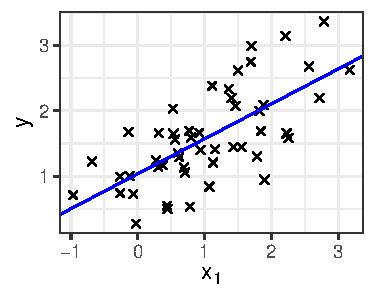
\includegraphics[width=\textwidth]{figure/reg_l2_basic_lm.pdf} 
\end{minipage}
\hspace{1cm}
\begin{minipage}{0.4\textwidth}
    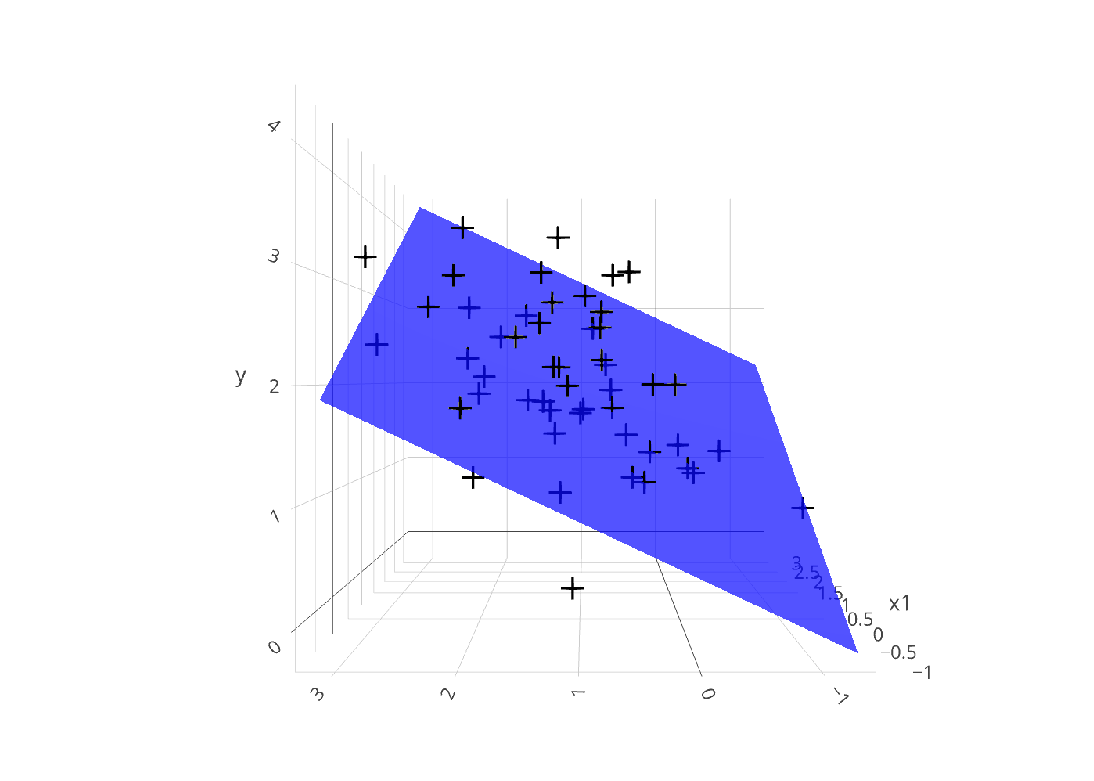
\includegraphics[width=1.2\textwidth, trim=100 0 0 20, clip]{
    figure/reg_l2_basic_lm_biv.pdf} 
\end{minipage}

\end{vbframe} 

% ------------------------------------------------------------------------------

\begin{vbframe}{Model fit with l2 loss}

\begin{itemize}
    \item How to determine parameters that specify the linear model? $\rightsquigarrow$ define loss function \& optimize risk
    \item Popular loss function for linear regression: \textbf{$L2$ loss} / \textbf{quadratic loss} / 
    \textbf{squared error}
    $$\Lxy = (y - \yh)^2 = (y-\fx)^2 = (y-\thx)^2$$
    
    % 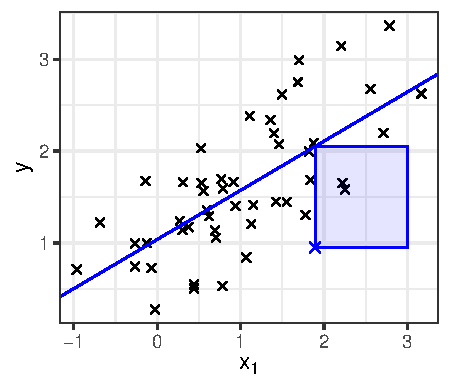
\includegraphics[width=0.35\textwidth]{figure/reg_l2_residual.pdf}
    % diese Grafik ist irgendwie verwirrend, weil es so aussieht, als 
    % wäre das Kästchen ein Rechteck und kein Quadrat
    \item The difference between the observed value $y$ and the estimated value $\yh = \fx$ is known as a \textbf{residual} and denoted by $r = y - \fx$
    \item By choosing the $L2$ loss, the residuals are penalized \textbf{quadratically}
    \item Reasons for choosing the $L2$ loss:
    \begin{itemize}
        \item Easy to optimize (convex, differentiable)
        \item Theoretically appealing characteristics 
        \item Connection to classical stats LM
    \end{itemize}
\end{itemize}

\end{vbframe}

% ------------------------------------------------------------------------------

\begin{vbframe}{l2 loss plots}

We will often visualize loss effects like this:

\vfill

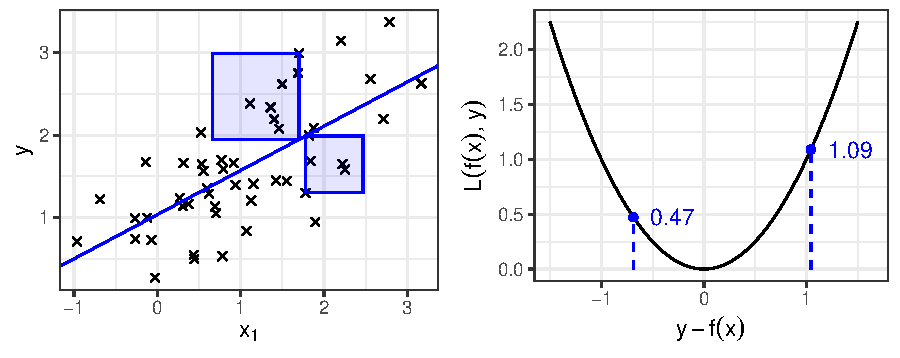
\includegraphics[width=\textwidth]{figure/reg_l2_lossplot_quad.pdf}

\hspace{0.5cm}
\begin{minipage}[t]{0.45\textwidth}
    \footnotesize
    \begin{itemize}
        \item Data as $y \sim x_1$
        % \item Prediction hypersurface \\$\rightsquigarrow$ here: line
        \item Residuals \textcolor{blue}{$r = y - \fx$}
        \\$\rightsquigarrow$ squares to illustrate loss
    \end{itemize}
\end{minipage}
\hfill
\begin{minipage}[t]{0.4\textwidth}
    \footnotesize
    \begin{itemize}
        \item Loss as function of residuals
        %\\$\rightsquigarrow$ strength of penalty? 
        %\\$\rightsquigarrow$ symmetric?
        \item Highlighted: loss for residuals shown on LHS
    \end{itemize}
\end{minipage}

\end{vbframe}

% ------------------------------------------------------------------------------

\begin{vbframe}{analytical optimization with l2 loss}

\begin{itemize}
    \item With the L2 loss, the resulting \textbf{risk} is:
    $$\risket = \sumin \left(\yi - \thetab^\top \xi \right)^2$$
    \item This is equivalent to the \textbf{sum of squared errors (SSE)}
    \item By minimizing the sum of the quadratic differences between $y$ and $\yh$, we find the loss-optimal model
    \item Special property of LM with $L2$ loss: \textbf{analytical solution} available
    \begin{align*}
        \thetabh \in 
        \argmin_{\thetab} \risket &=
        \argmin_{\thetab} \sumin \left(\yi - \thetab^\top \xi \right)^2  %\\
        % &= \argmin_{\thetab} \| \yv - \Xmat \thetab \|^2_2
    \end{align*}
    \normalsize
    \item The solution $\thetabh$ is known as the \textbf{ordinary-least-squares (OLS)} estimator and we can find it via \textbf{normal equations}
\end{itemize}

\end{vbframe}

% ------------------------------------------------------------------------------

\begin{vbframe}{Statistical properties l2 loss}

% \footnotesize
\begin{itemize}
    % \small
    % \item In a nutshell: minimize quadratic residuals of form 
    % $\| \yv - \Xmat \thetab \|^2_2$
    \item LM with $L2$ loss intimately related to classical stats LM
    \item Assumptions
    \begin{itemize}
        % \small
        \item $\xi$ \textbf{i}ndependent and \textbf{i}dentically \textbf{d}istributed \textbf{(iid)} for $i \in \nset$
        \item \textbf{Homoskedastic} (equivariant) 
         \textbf{Gaussian} errors
        $$\yv = \Xmat \thetab + \bm{\epsilon}, ~ \bm{\epsilon} \sim 
        \normal(0, \sigma^2 \id)  $$
        $\rightsquigarrow$ $y_i$ conditionally independent \& normally ditributed
        % $\yv | \Xmat \sim \normal(\Xmat \thetab, \sigma^2 \id)$
        \item \textbf{Uncorrelated features} \\$\rightsquigarrow$ 
        multicollinearity destabilizes effect estimation 
    \end{itemize}
    \item If assumptions hold: statistical \textbf{inference} applicable
    \begin{itemize}
        % \small
            \item Hypothesis tests on significance of effects, incl. $p$-values
            \item Confidence \& prediction intervals via student-$t$ 
            distribution
        \item Goodness-of-fit measure
        $R^2 = 1 - \text{SSE} ~~ / \underbrace{\text{SST}}_{
        \sumin (\yi - \bar y)^2}$
        
        $\rightsquigarrow$ SSE = part of data variance \textit{not} explained 
        by model
    \end{itemize}
\end{itemize}

\end{vbframe}

% ------------------------------------------------------------------------------

\begin{vbframe}{Effect interpretation - ans Ende setzen, ist für l1 und l2 loss gleich}

\begin{itemize}
    \item Big plus of LM: immediately \textbf{interpretable} feature effects
    \item "Marginally increasing $x_j$ by 1 unit increases $y$ by $\theta_j$ 
    units" \\
    $\rightsquigarrow$ \textit{ceteris paribus} assumption: 
    $x_1, \dots, x_{j - 1}, x_{j + 1}, \dots, x_p$ fixed
\end{itemize}

\vfill
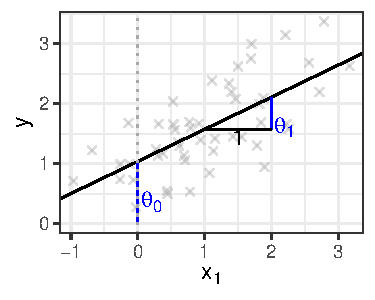
\includegraphics[width=0.4\textwidth]{figure/reg_l2_basic_lm_interpreted.pdf} 
\hfill
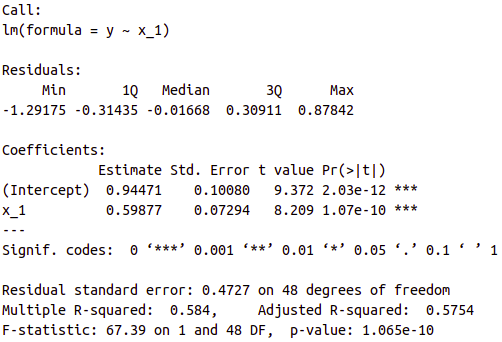
\includegraphics[width=0.55\textwidth]{figure_man/lm_summary} 

\end{vbframe}

% ------------------------------------------------------------------------------


\begin{vbframe}{Ab hier vollumfängliche Folien reinkopiert}

\end{vbframe}

% ------------------------------------------------------------------------------

\begin{vbframe}{Design matrix}

\begin{itemize}
    \item Mismatch: $\thetab \in \R^{p + 1}$ vs $\xv \in \R^p$ due to intercept  
    term
    \item Trick: pad feature vectors with leading 1, s.t. 
    \begin{itemize}
        \item $\xv \mapsto \xv = (1, x_1, \dots, x_p)^\top$, and 
        \item $\thx = \theta_0 \cdot 1 + \theta_1 x_1 + \dots + \theta_p x_p$
    \end{itemize}
    \item Collect all observations in \textbf{design matrix} 
    $\Xmat \in \R^{n \times (p + 1)}$ \\
    $\rightsquigarrow$ more compact: single param vector incl. intercept
    \item Resulting linear model:
    \begin{align*}
    \hat \yv = \Xmat \thetab = 
        \left(
        \begin{smallmatrix}
            1 & x^{(1)}_1 & \ldots & x^{(1)}_p \\
            1 & x^{(2)}_1 & \ldots & x^{(2)}_p \\
            \vdots & \vdots & & \vdots \\
            1 & x^{(n)}_1 & \ldots & x^{(n)}_p \\
        \end{smallmatrix}
        \right)
        \left(
        \begin{smallmatrix}
            \theta_0 \\ \theta_1 \\ \vdots \\ \theta_p
        \end{smallmatrix}
        \right)
        &=
        \left(
        \begin{smallmatrix}
            \theta_0 + \theta_1 x_1^{(1)} + \dots + \theta_p x_p^{(1)} \\
            \theta_0 + \theta_1 x_1^{(2)} + \dots + \theta_p x_p^{(2)} \\
            \vdots \\
            \theta_0 + \theta_1 x_1^{(n)} + \dots + \theta_p x_p^{(n)} \\
        \end{smallmatrix}
        \right)
    \end{align*}
    \item We will make use of this notation in other contexts
\end{itemize}

\end{vbframe}

% ------------------------------------------------------------------------------

\begin{vbframe}{Effect interpretation}

\begin{itemize}
    \item Big plus of LM: immediately \textbf{interpretable} feature effects
    \item "Marginally increasing $x_j$ by 1 unit increases $y$ by $\theta_j$ 
    units" \\
    $\rightsquigarrow$ \textit{ceteris paribus} assumption: 
    $x_1, \dots, x_{j - 1}, x_{j + 1}, \dots, x_p$ fixed
\end{itemize}

\vfill
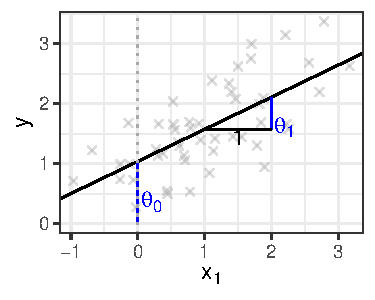
\includegraphics[width=0.4\textwidth]{figure/reg_l2_basic_lm_interpreted.pdf} 
\hfill
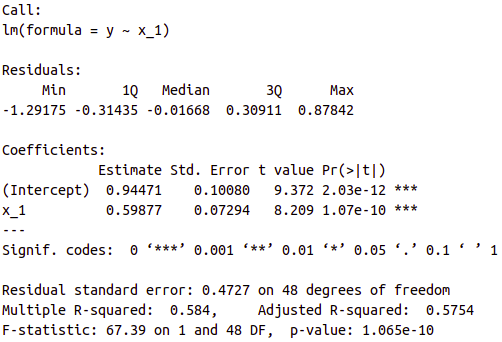
\includegraphics[width=0.55\textwidth]{figure_man/lm_summary} 

\end{vbframe}

% ------------------------------------------------------------------------------

\begin{frame}{Model fit}

\begin{itemize}
    \item How to determine LM fit? $\rightsquigarrow$ define risk \& optimize
    \item Popular: \textbf{$L2$ loss} / \textbf{quadratic loss} / 
    \textbf{squared error}
    $$\Lxy = (y-\fx)^2 ~~ \text{or} ~~ \Lxy = 0.5 \cdot (y-\fx)^2$$
    
    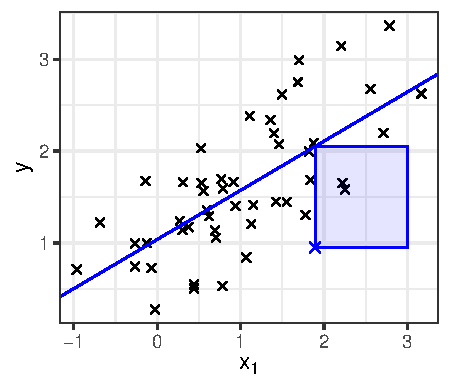
\includegraphics[width=0.35\textwidth]{figure/reg_l2_residual.pdf}
    \item Why penalize \textbf{residuals} $r = y - \fx$ quadratically?
    \begin{itemize}
        \item Easy to optimize (convex, differentiable)
        \item Theoretically appealing (connection to classical stats LM)
    \end{itemize}
\end{itemize}

\end{frame}

% ------------------------------------------------------------------------------

\begin{frame}{loss plots}

We will often visualize loss effects like this:

\vfill

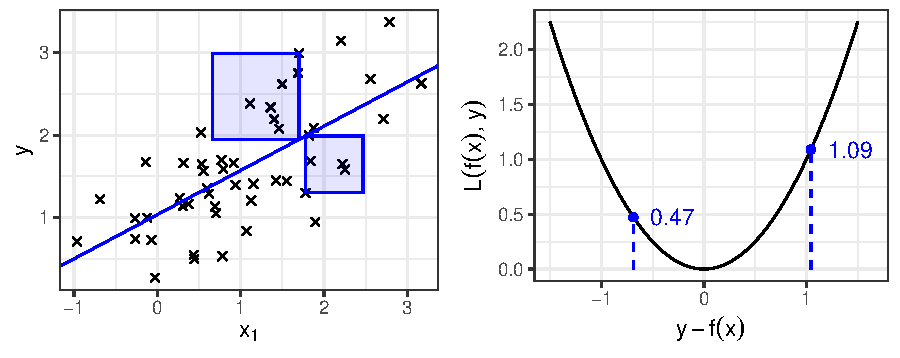
\includegraphics[width=\textwidth]{figure/reg_l2_lossplot_quad.pdf}

\hspace{0.5cm}
\begin{minipage}[t]{0.45\textwidth}
    \footnotesize
    \begin{itemize}
        \item Data as $y \sim x_1$
        \item Prediction hypersurface \\$\rightsquigarrow$ here: line
        \item Residuals \textcolor{blue}{$r = y - \fx$}
        \\$\rightsquigarrow$ squares to illustrate loss
    \end{itemize}
\end{minipage}
\hfill
\begin{minipage}[t]{0.4\textwidth}
    \footnotesize
    \begin{itemize}
        \item Loss as function of residuals
        \\$\rightsquigarrow$ strength of penalty? 
        \\$\rightsquigarrow$ symmetric?
        \item Highlighted: loss for residuals shown on LHS
    \end{itemize}
\end{minipage}

\end{frame}

% ------------------------------------------------------------------------------

\begin{frame}{optimization}

\begin{itemize}
    \item Resulting risk equivalent to 
    \textbf{sum of squared errors (SSE)}:
    $$\risket = \sumin \left(\yi - \thetab^\top \xi \right)^2$$
    \item Consider example with $n = 5$ $\rightsquigarrow$ 
    different models with varying SSE
\end{itemize}

\vfill
\only<1>{
    \phantom{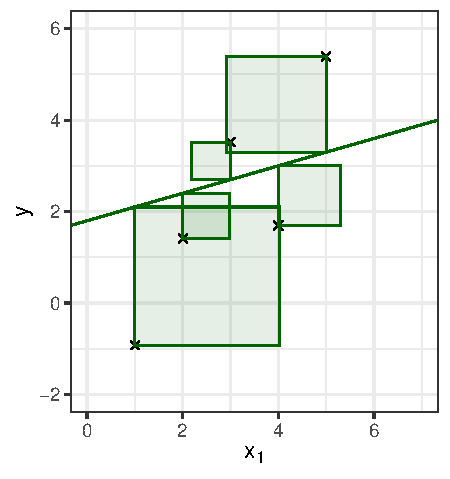
\includegraphics[width=0.25\textwidth]{
    figure/reg_l2_sse_1.pdf}}
}
\only<2>{
    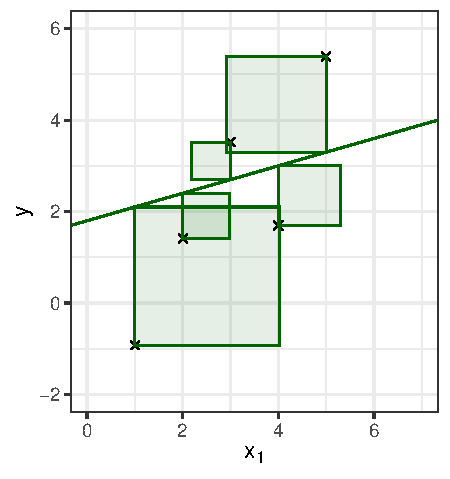
\includegraphics[width=0.3\textwidth]{figure/reg_l2_sse_1.pdf}
}
\only<3>{
    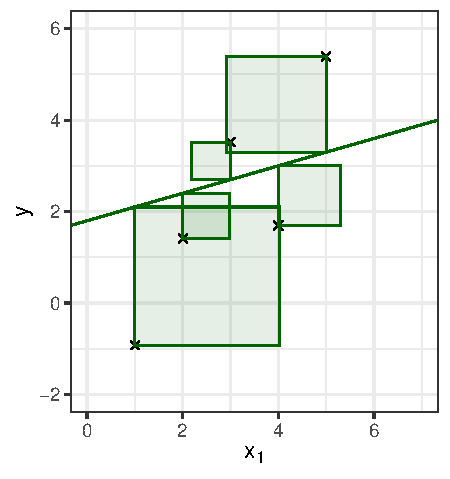
\includegraphics[width=0.3\textwidth]{figure/reg_l2_sse_1.pdf}
    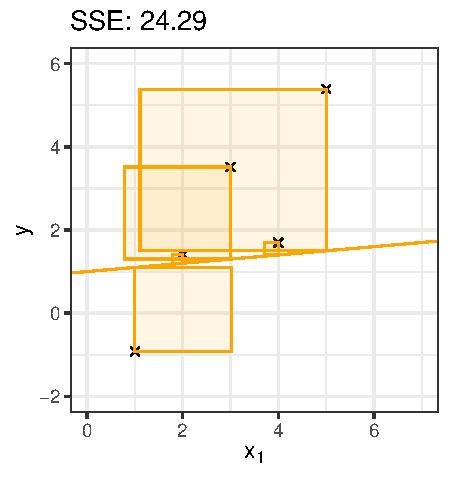
\includegraphics[width=0.3\textwidth]{figure/reg_l2_sse_2.pdf}
}
\only<4>{
    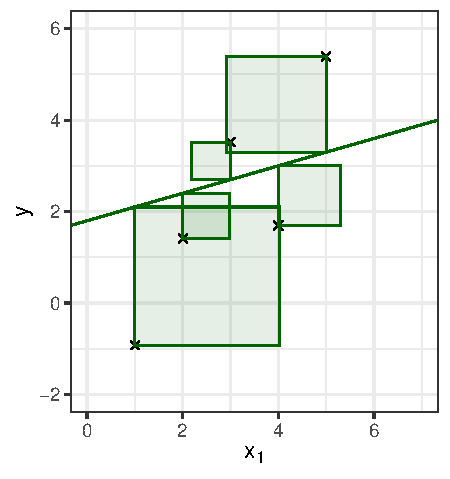
\includegraphics[width=0.3\textwidth]{figure/reg_l2_sse_1.pdf}
    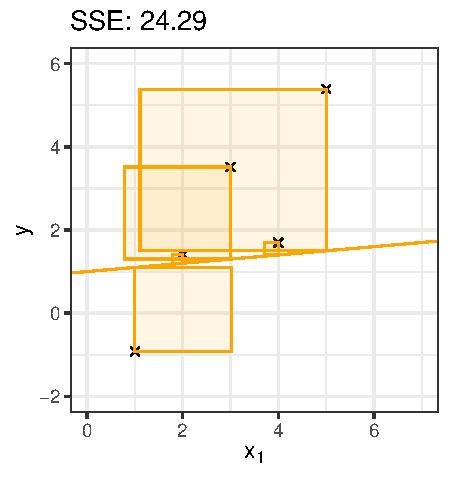
\includegraphics[width=0.3\textwidth]{figure/reg_l2_sse_2.pdf}
    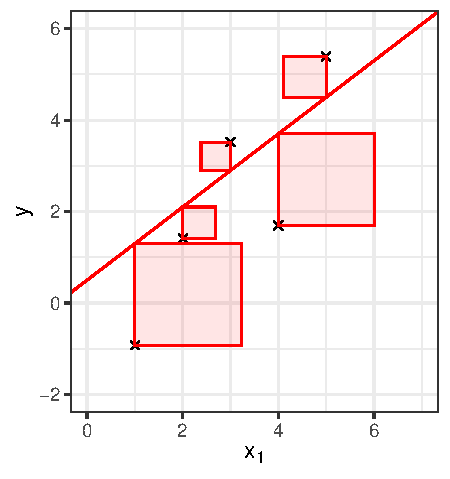
\includegraphics[width=0.3\textwidth]{figure/reg_l2_sse_3.pdf}
}

\end{frame}

% ------------------------------------------------------------------------------

\begin{frame}{optimization}

% Only stuff below super tedious, but when leaving out the repetitions (defining
% table globally and only adding lines in only statements), there's weird
% indenting...

\vspace{0.2cm}
\begin{minipage}[c]{0.5\textwidth}
    % \only<1>{
    % 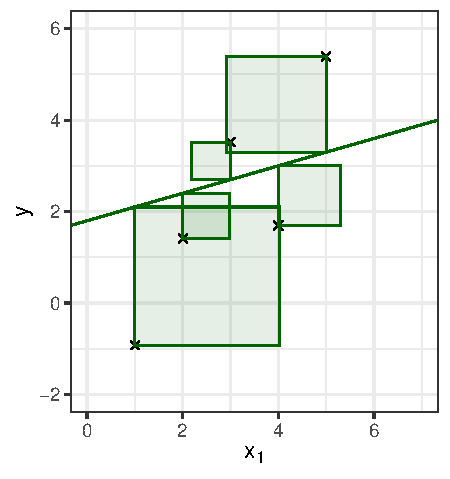
\includegraphics[width=0.4\textwidth]{figure/reg_l2_sse_1.pdf} \\
    % \phantom{
    %     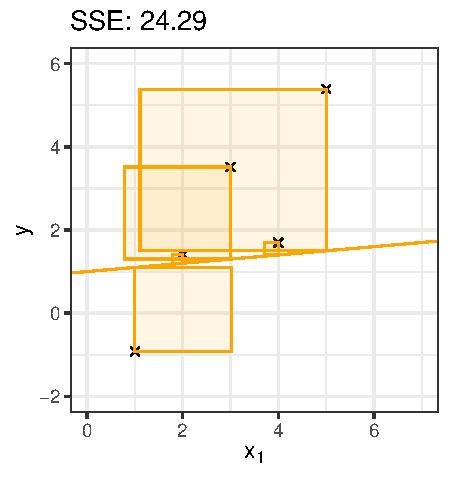
\includegraphics[width=0.4\textwidth]{figure/reg_l2_sse_2.pdf} \\
    % }
    % \phantom{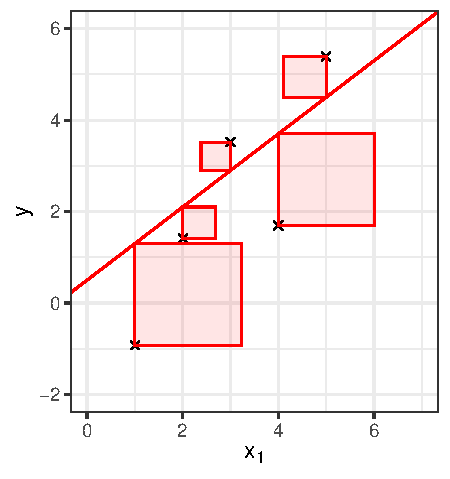
\includegraphics[width=0.4\textwidth]{figure/reg_l2_sse_3.pdf}}
    % \vfill \vspace{0.5cm} \scriptsize
    % \begin{tabular}{r|r|r}
    %     Intercept $\theta_0$ & Slope $\theta_1$ & SSE
    %     \\ \hline 1.80 & 0.30 & 16.86\\ \hline && \\ \hline && \\ \hline &&
    % \end{tabular}
    % }
    % \only<2>{
    % 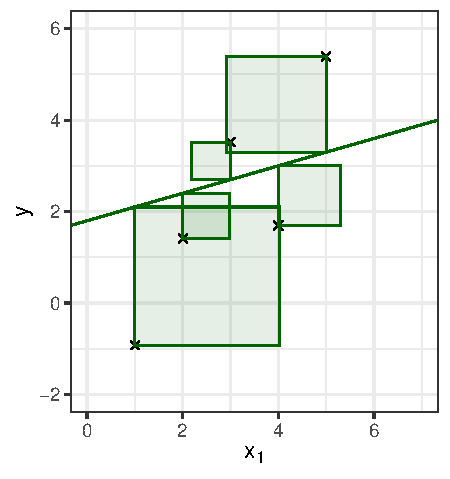
\includegraphics[width=0.4\textwidth]{figure/reg_l2_sse_1.pdf}
    % 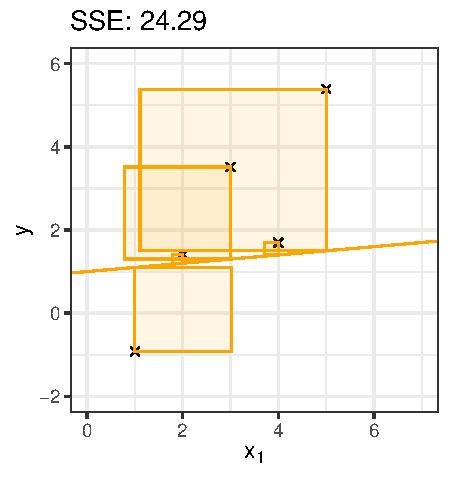
\includegraphics[width=0.4\textwidth]{figure/reg_l2_sse_2.pdf} \\
    % \phantom{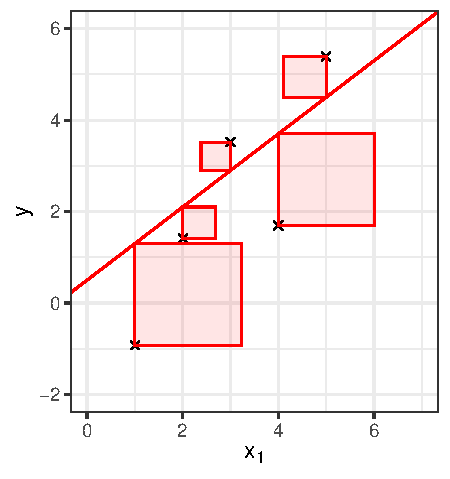
\includegraphics[width=0.4\textwidth]{figure/reg_l2_sse_3.pdf}}
    % \vfill \vspace{0.5cm} \scriptsize
    % \begin{tabular}{r|r|r}
    %     Intercept $\theta_0$ & Slope $\theta_1$ & SSE
    %     \\ \hline 1.80 & 0.30 & 16.86\\ \hline 1.00 & 0.10 & 24.29 \\ 
    %     \hline && \\ \hline &&
    % \end{tabular}
    % }
    \only<1>{
    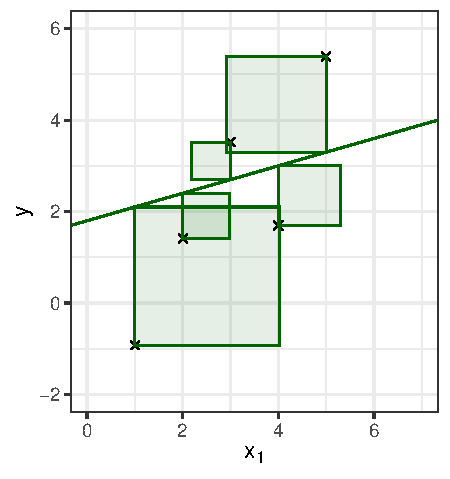
\includegraphics[width=0.4\textwidth]{figure/reg_l2_sse_1.pdf}
    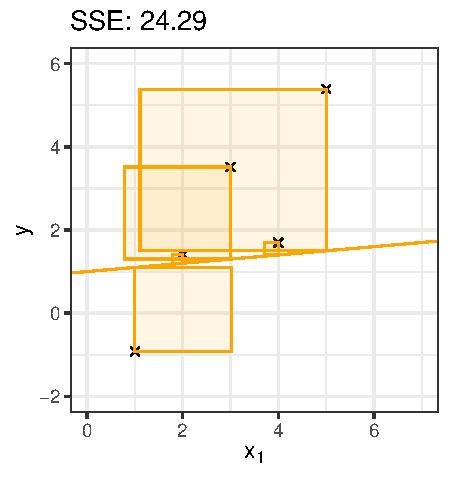
\includegraphics[width=0.4\textwidth]{figure/reg_l2_sse_2.pdf} \\
    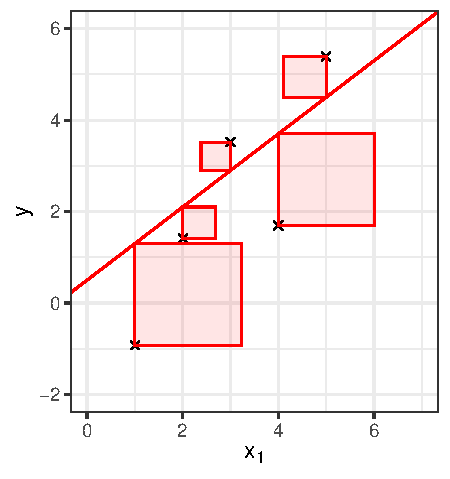
\includegraphics[width=0.4\textwidth]{figure/reg_l2_sse_3.pdf}
    \vfill \vspace{0.5cm} \scriptsize
    \begin{tabular}{r|r|r}
        Intercept $\theta_0$ & Slope $\theta_1$ & SSE
        \\ \hline 1.80 & 0.30 & 16.86\\ \hline 1.00 & 0.10 & 24.29 \\
        \hline 0.50 & 0.80 & 10.61 \\ \hline &&
    \end{tabular}
    }
    \only<2>{
    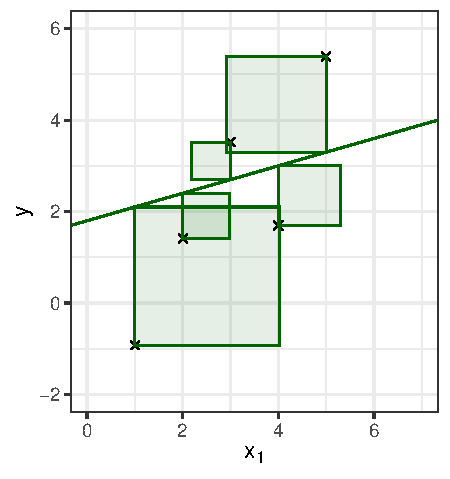
\includegraphics[width=0.4\textwidth]{figure/reg_l2_sse_1.pdf}
    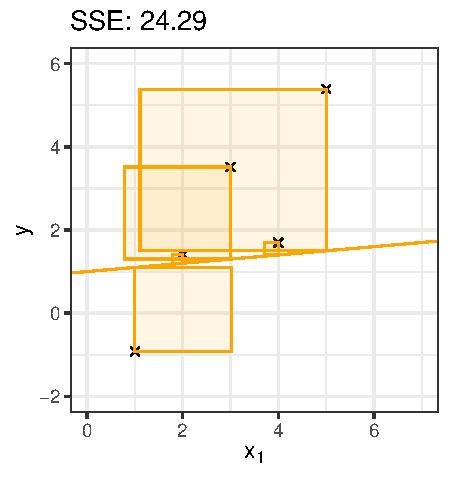
\includegraphics[width=0.4\textwidth]{figure/reg_l2_sse_2.pdf} \\
    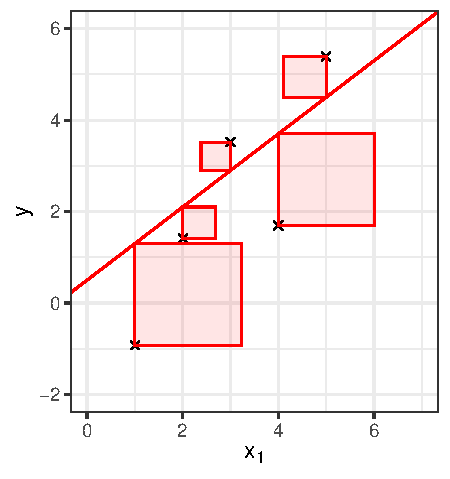
\includegraphics[width=0.4\textwidth]{figure/reg_l2_sse_3.pdf}
    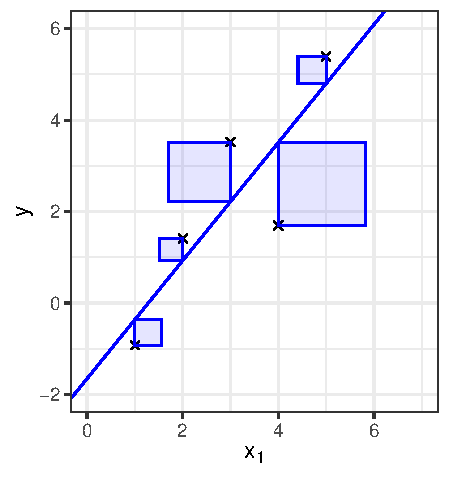
\includegraphics[width=0.4\textwidth]{figure/reg_l2_sse_4.pdf}
    \vfill \vspace{0.5cm} \scriptsize
    \begin{tabular}{r|r|r}
        Intercept $\theta_0$ & Slope $\theta_1$ & SSE
        \\ \hline 1.80 & 0.30 & 16.86\\ \hline 1.00 & 0.10 & 24.29 
        \\ \hline 0.50 & 0.80 & 10.61 \\ \hline
        \textcolor{blue}{-1.65} & \textcolor{blue}{1.29} &
        \textcolor{blue}{5.88}
    \end{tabular}
    }
\end{minipage}
\begin{minipage}[c]{0.45\textwidth}
    % \only<1>{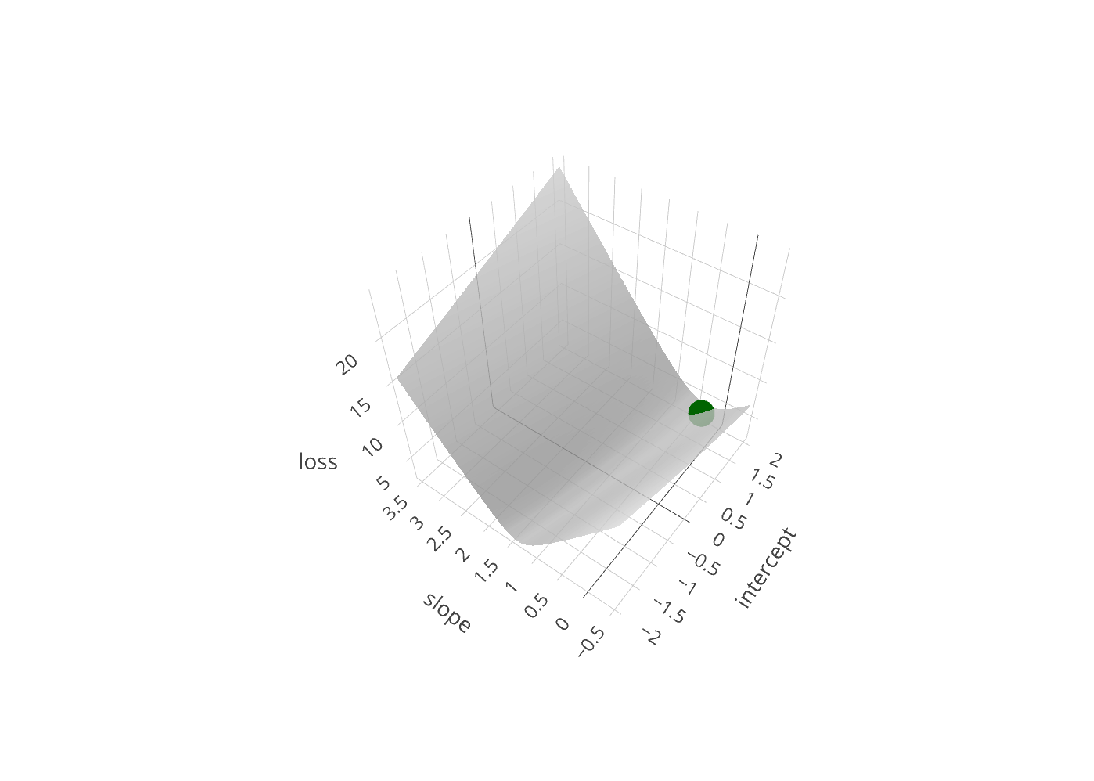
\includegraphics[width=1.2\textwidth, trim=130 30 80 20, clip]{
    % figure/reg_l2_sse_optim_1.pdf}}
    % \only<2>{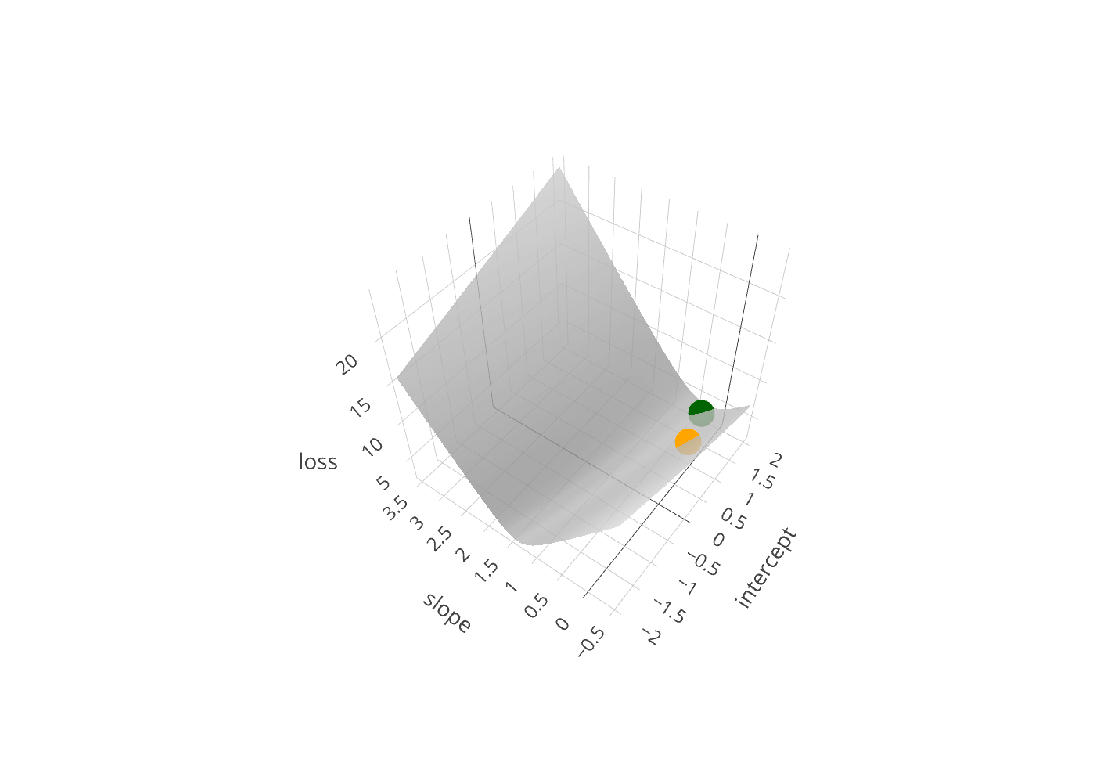
\includegraphics[width=1.2\textwidth, trim=130 30 80 20, clip]{
    % figure/reg_l2_sse_optim_2.pdf}}
    \only<1>{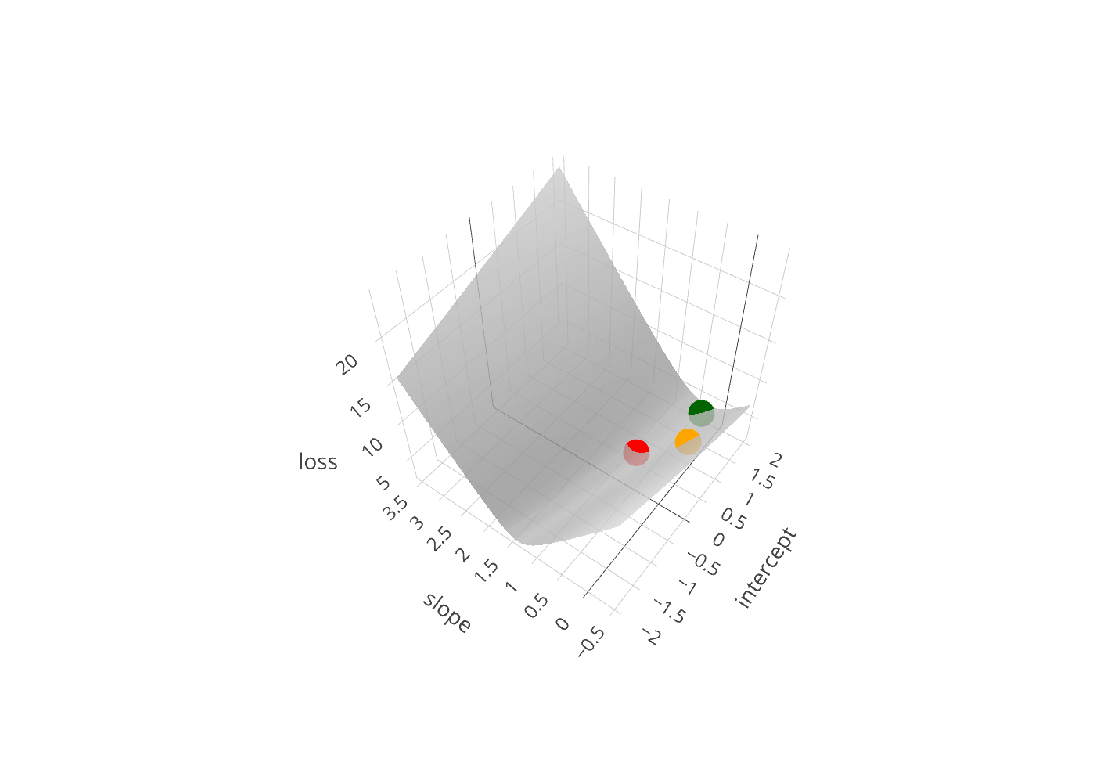
\includegraphics[width=1.2\textwidth, trim=130 30 80 20, clip]{
    figure/reg_l2_sse_optim_3.pdf}}
    \only<2>{
    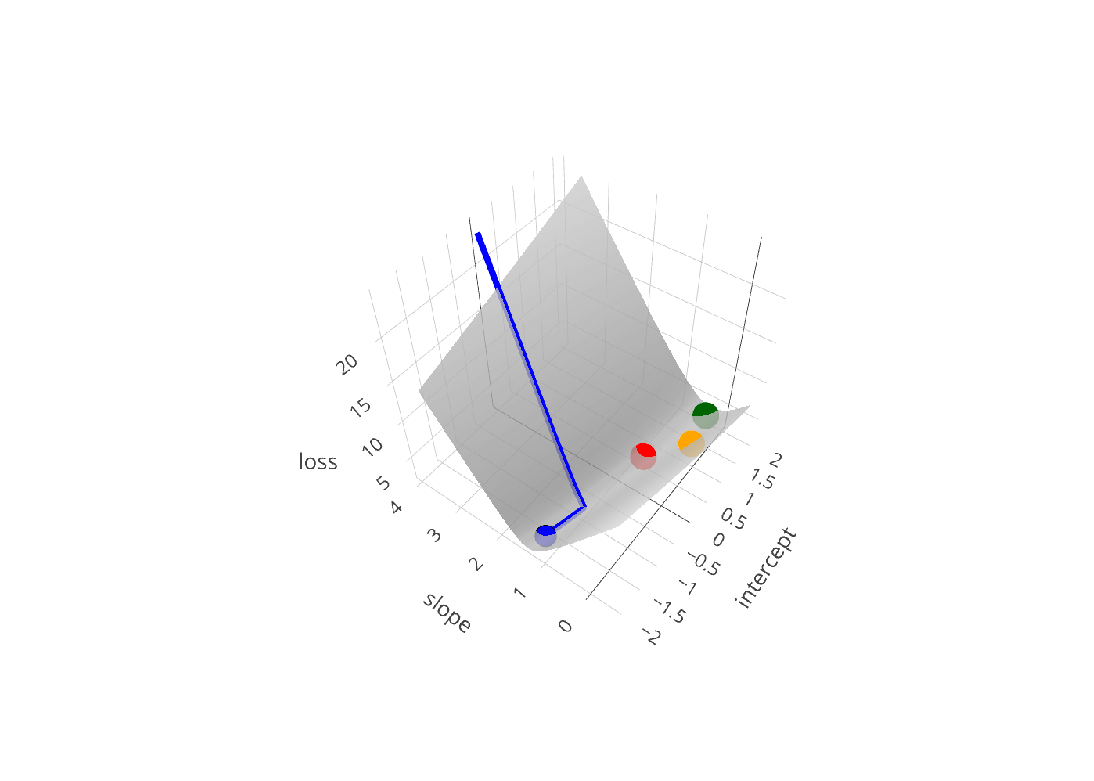
\includegraphics[width=1.2\textwidth, trim=130 10 80 20, clip]{
    figure/reg_l2_sse_optim_4.pdf}}
\end{minipage}

\only<2>{
\vfill

Instead of guessing, of course, use \textbf{optimization}!
}

\end{frame}

% ------------------------------------------------------------------------------

\begin{vbframe}{analytical optimization}

\begin{itemize}
    \item Special property of LM with $L2$ loss: \textbf{analytical solution}
    available
    \begin{align*}
        \thetabh \in 
        \argmin_{\thetab} \risket &=
        \argmin_{\thetab} \sumin \left(\yi - \thetab^\top \xi \right)^2  \\
        &= \argmin_{\thetab} \| \yv - \Xmat \thetab \|^2_2
    \end{align*}
    \normalsize
    \item Find via \textbf{normal equations}
    $$\pd{\risket}{\thetab} = 0$$
    \item Solution: \textbf{ordinary-least-squares (OLS)} estimator
    $$\thetabh = \olsest$$
\end{itemize}

\end{vbframe}

% ------------------------------------------------------------------------------

\begin{vbframe}{Statistical properties}

% \footnotesize
\begin{itemize}
    % \small
    % \item In a nutshell: minimize quadratic residuals of form 
    % $\| \yv - \Xmat \thetab \|^2_2$
    \item LM with $L2$ loss intimately related to classical stats LM
    \item Assumptions
    \begin{itemize}
        % \small
        \item $\xi$ \textbf{iid} for $i \in \nset$
        \item \textbf{Homoskedastic} (equivariant) 
         \textbf{Gaussian} errors
        $$\yv = \Xmat \thetab + \bm{\epsilon}, ~ \bm{\epsilon} \sim 
        \normal(0, \sigma^2 \id)  $$
        $\rightsquigarrow$ $y_i$ conditionally independent \& normal:
        $\yv | \Xmat \sim \normal(\Xmat \thetab, \sigma^2 \id)$
        \item Uncorrelated features \\$\rightsquigarrow$ 
        multicollinearity destabilizes effect estimation 
    \end{itemize}
    \item If assumptions hold: statistical \textbf{inference} applicable
    \begin{itemize}
        % \small
            \item Hypothesis tests on significance of effects, incl. $p$-values
            \item Confidence \& prediction intervals via student-$t$ 
            distribution
        \item Goodness-of-fit measure
        $R^2 = 1 - \text{SSE} ~~ / \underbrace{\text{SST}}_{
        \sumin (\yi - \bar y)^2}$
        
        $\rightsquigarrow$ SSE = part of data variance \textit{not} explained 
        by model
    \end{itemize}
\end{itemize}

\end{vbframe}

%%%%%%%%%%%%%%%%%%%%%%%%%%%%%%%%%%%%%%%%%%%
%%%% deep dive OLS regression raus

%%%%%%%%%%%%%%%%%%%%%%%%%%%%%%%%%%%%%%%%%%%%%%%%%%%
%%%%%% L1
%%%%%%%%%%%%%%%%%%%%%%%%%%%%%%%%%%%%%%%%%%%%%%%%%%%

\begin{vbframe}{Absolute loss}

\begin{itemize}
    \item $L2$ regression minimizes quadratic residuals -- wouldn't 
    \textbf{absolute} residuals seem more natural? 
    \vspace{0.2cm}
    \begin{center}
    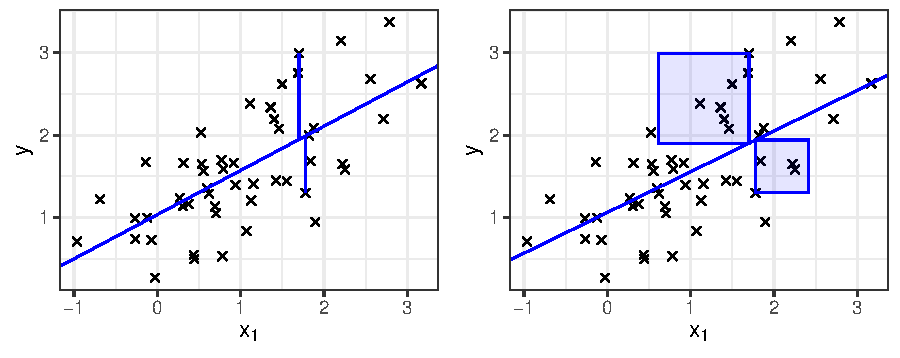
\includegraphics[width=0.55\textwidth]{figure/reg_l1_residual_abs_vs_quad}
    \end{center}
    \item \textbf{$L1$ loss / absolute error / least absolute deviation (LAD)}
    $$\Lxy = |y - \fx|$$
    \begin{center}
    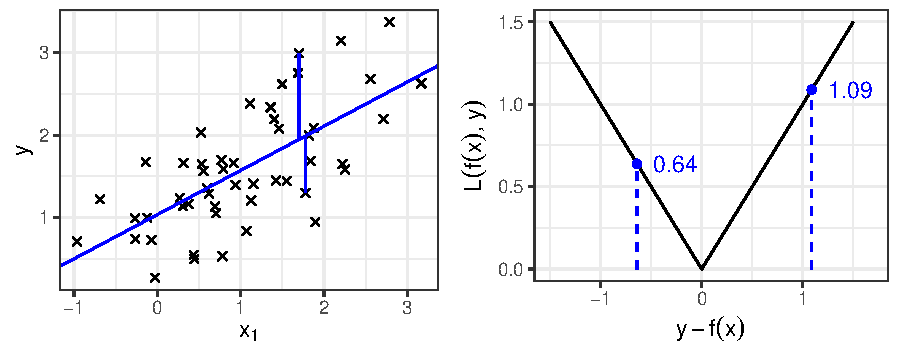
\includegraphics[width=0.55\textwidth]{figure/reg_l1_lossplot_abs}
    \end{center}
\end{itemize}

\end{vbframe}

% ------------------------------------------------------------------------------

\begin{vbframe}{$L1$ vs $L2$ -- loss surface}

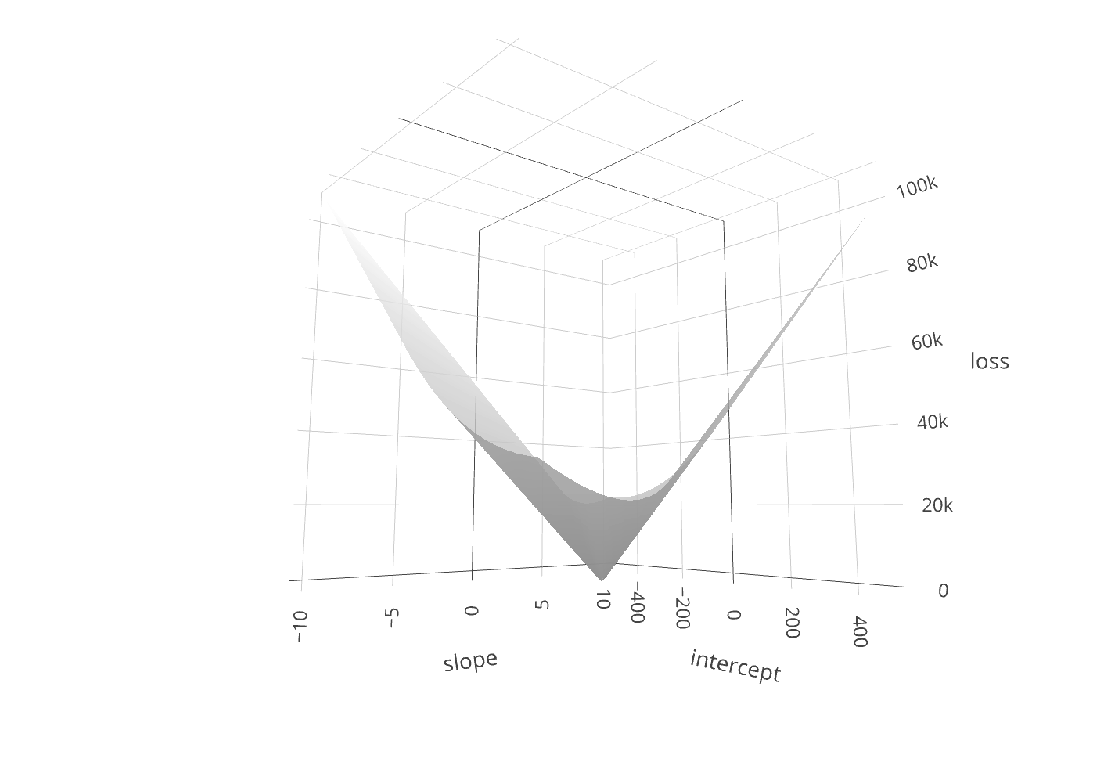
\includegraphics[width=0.49\textwidth, trim=100 30 100 0, clip]{
figure/reg_l1_surface_abs.pdf}
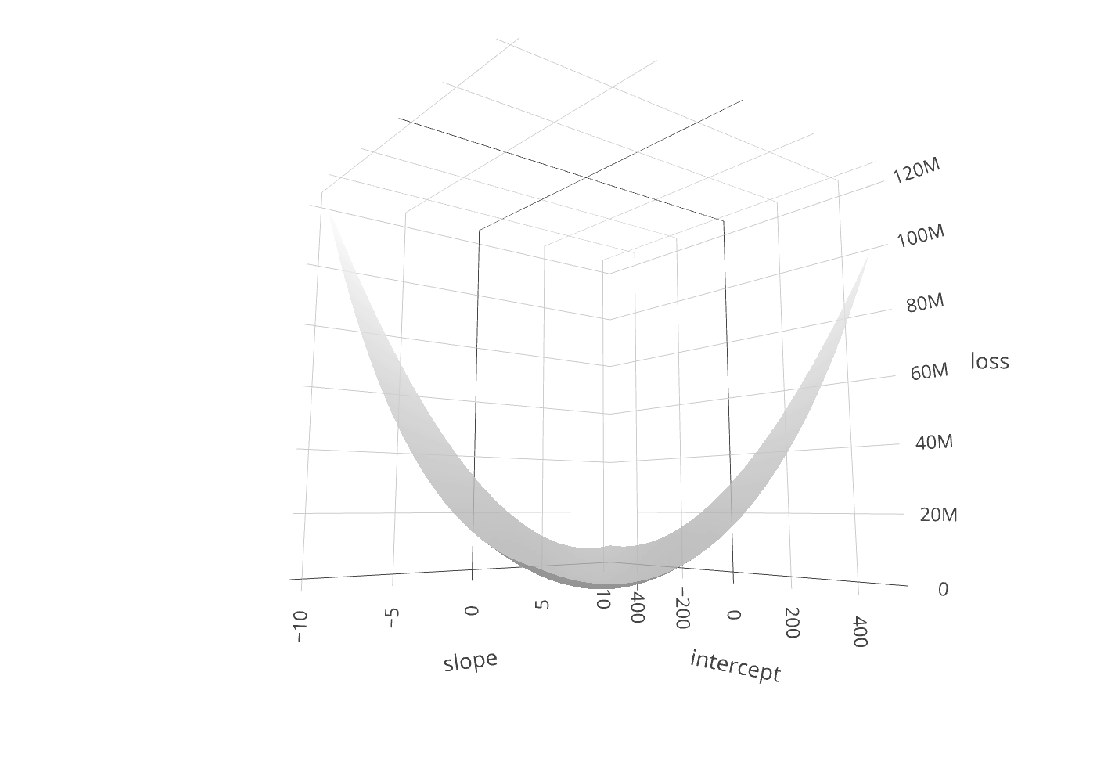
\includegraphics[width=0.49\textwidth, trim=100 30 100 0, clip]{
figure/reg_l1_surface_quad.pdf}
\vfill

$L1$ loss (left) harder to optimize than $L2$ loss (right)
\begin{itemize}
    \item Convex but \textbf{not differentiable} in
    $y - \fx = 0$
    \item No analytical solution
\end{itemize}

\end{vbframe}

% ------------------------------------------------------------------------------

\begin{vbframe}{$L1$ vs $L2$ -- estimated parameters}

\begin{itemize}
    \item Results of $L1$ and $L2$ regression often not that different
    \item Simulated data: $\yi = 1 + 0.5 x^{(i)}_1 + \epsi$, ~~ $\epsi \iid
    \normal(0, 0.01)$
    % \item Coefficients:
\end{itemize}
    
\vfill

\begin{minipage}[b]{0.65\textwidth}
    \hspace{0.7cm}
    \footnotesize
    \begin{tabular}{r|r|r}
        & intercept & slope \\ \hline
        \textcolor{blue}{$L1$} & 0.91 & 0.53 \\ \hline
        \textcolor{orange}{$L2$} & 0.91 & 0.57 
    \end{tabular}

    \vspace{0.5cm}
    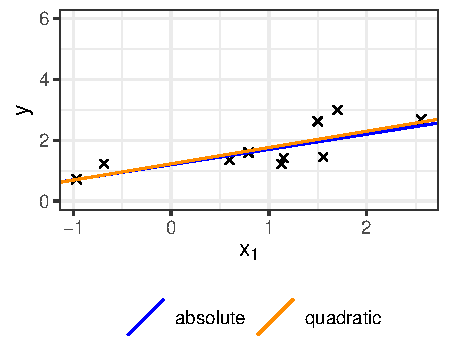
\includegraphics[width=0.8\textwidth]{figure/reg_l1_comparison.pdf}
\end{minipage}
\begin{minipage}[b]{0.34\textwidth}
    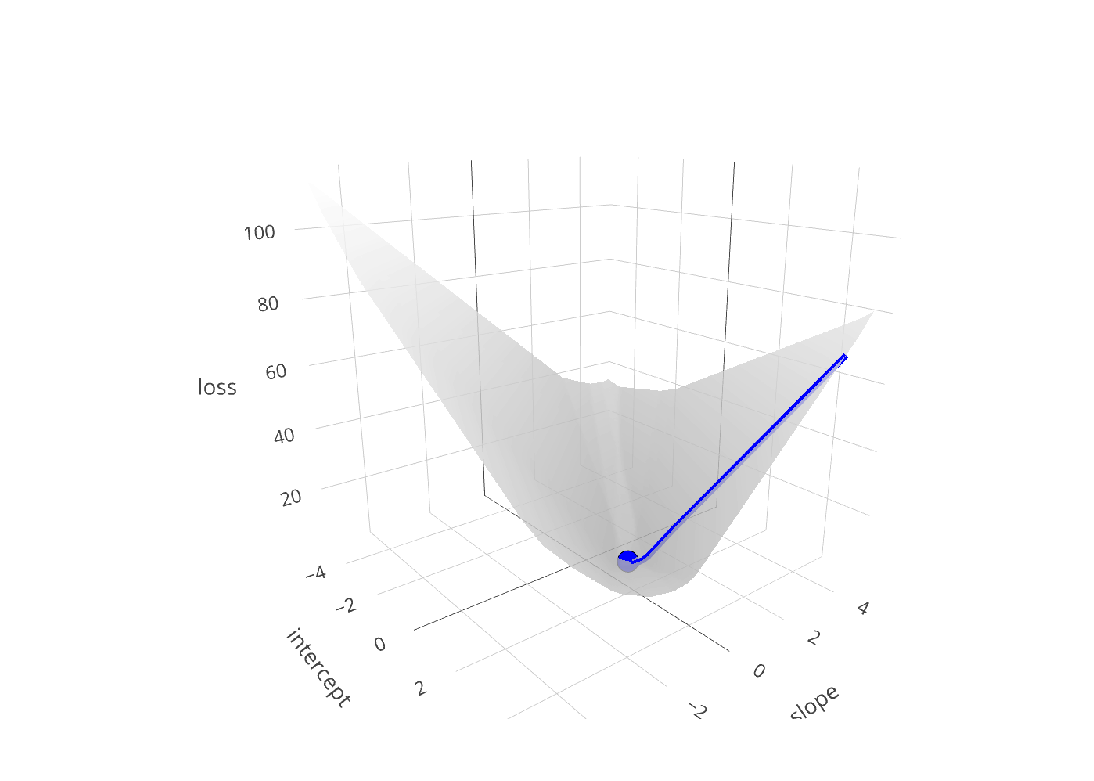
\includegraphics[width=\textwidth, trim=80 0 100 80, clip]{
    figure/reg_l1_comparison_optim_abs.pdf}
    
    \vfill
    
    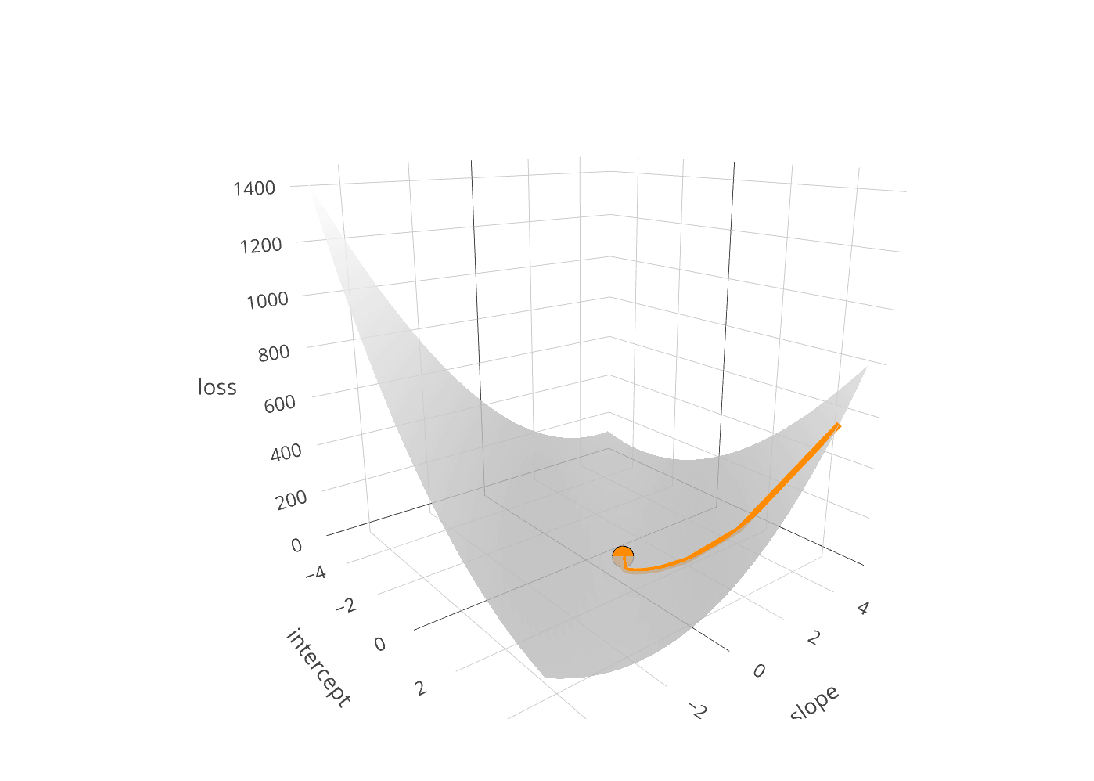
\includegraphics[width=\textwidth, trim=80 0 100 80, clip]{
    figure/reg_l1_comparison_optim_quad.pdf}
\end{minipage}

\end{vbframe}

% ------------------------------------------------------------------------------

\begin{vbframe}{$L1$ vs $L2$ -- robustness}

\begin{itemize}
    \item $L2$ quadratic in residuals $\rightsquigarrow$ outlying points 
    carry lots of weight
    \item E.g., $3 \times$ residual $\Rightarrow$ $9 \times$ loss contribution
    \item $L1$ more \textbf{robust} in presence of outliers (example ctd.):
\end{itemize}

\vfill
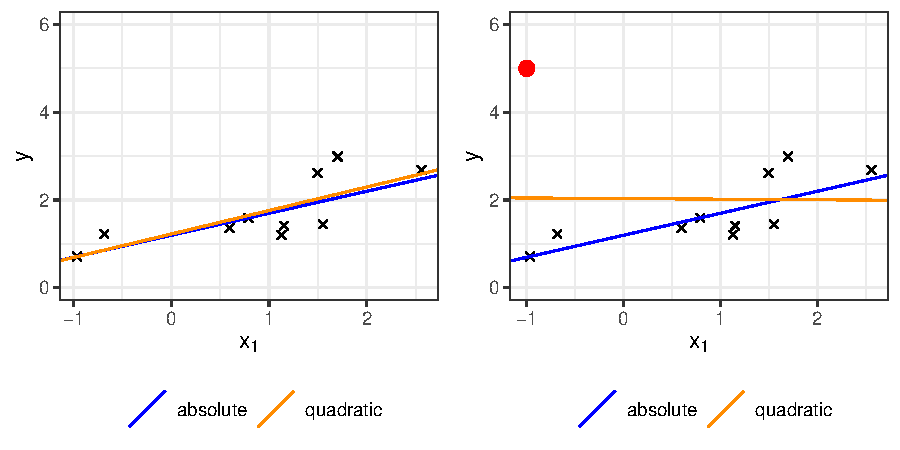
\includegraphics[width=\textwidth]{figure/reg_l1_comparison_outlier.pdf}

\end{vbframe}

% ------------------------------------------------------------------------------

\begin{vbframe}{$L1$ vs $L2$ -- optimization cost}

\begin{itemize}
    \item Real-world \texttt{weather} problem $\rightsquigarrow$ 
    predict mean temperature
    \item Compare \textbf{time} to fit $L1$ (\texttt{quantreg::rq()}) vs 
    $L2$ (\texttt{lm::lm()})
    for different dataset proportions (repeat $50\times$)
\end{itemize}

\vfill

\begin{minipage}[c]{0.54\textwidth}
    \centering
    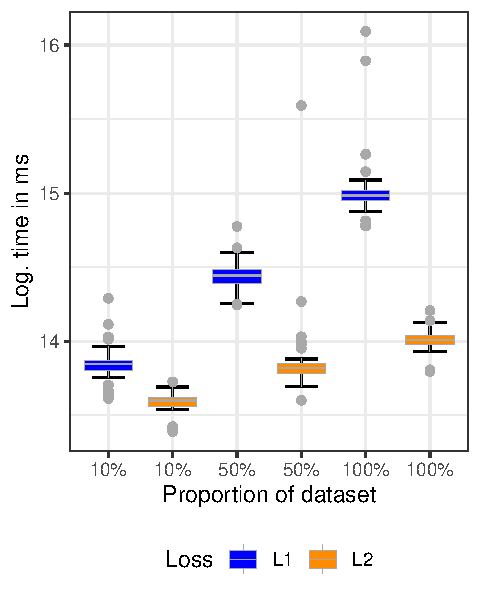
\includegraphics[width=0.8\textwidth]{figure/reg_l1_benchmark.pdf}
\end{minipage}
\scriptsize
\begin{minipage}[c]{0.45\textwidth}

    Loss
    
    \begin{tabular}{l|r|r}
        & Fitted: \textcolor{blue}{$L1$}  &
        Fitted: \textcolor{orange}{$L2$} \\ \hline
        Total \textcolor{blue}{$L1$} loss & $8.98 \times 10^4$ & 
        $8.99 \times 10^4$ \\
        Total \textcolor{orange}{$L2$} loss & $5.83 \times 10^6$ & 
        $5.81 \times 10^6$ \\
    \end{tabular}
    
    \vspace{0.5cm}
    
    Estimated coefficients \\
    
    \begin{tabular}{l|r|r}
        $x_j$ & \textcolor{blue}{$L1$: $\hat \theta_j$}  &
        \textcolor{orange}{$L2$: $\hat \theta_j$} \\ \hline
        \texttt{Max\_temperature} & 0.553 & 0.563 \\
        \texttt{Min\_temperature} & 0.441 & 0.427 \\
        \texttt{Visibility} & 0.026 & 0.041 \\
        \texttt{Wind\_speed} & 0.002 & 0.010 \\
        \texttt{Max\_wind\_speed} & $-$0.026 & $-$0.039 \\
        \texttt{(Intercept)} & $-$0.380 & $-$0.102 \\
    \end{tabular}
    
    \vspace{0.5cm}
    \normalsize
    $L1$ \textbf{slower} to optimize!
\end{minipage}

\end{vbframe}



%%%%%%%%%%%%%%%%%%%%%%%%%%%%%%%%%%%%%
%%%% POLYNOMIAL REGRESSION
%%%%%%%%%%%%%%%%%%%%%%%%%%%%%%%%%%%%%
%%% Eher raus denke ich

\lecturechapter{Supervised Regression:\\Polynomial Regression Models}
\lecture{Introduction to Machine Learning}

% ------------------------------------------------------------------------------

\begin{vbframe}{Increasing flexibility}

\begin{itemize}
    \item Recall our definition of LM: model $y$ as linear combo of features
    \item But: isn't that pretty \textbf{inflexible}?
    \item E.g., here, $y$ does not seem to be a linear function of $x$...

    \vspace{0.5cm}
    \begin{center}
        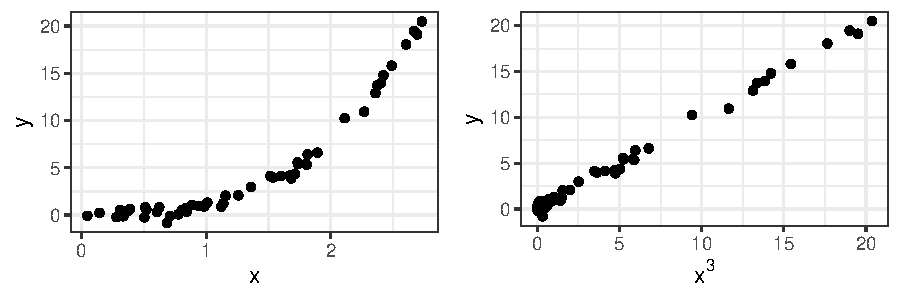
\includegraphics[width=0.6\textwidth]{figure/reg_poly_yx3.pdf}
    \end{center}

    ... but relation to $x^3$ looks pretty linear!

    \item Many other trafos conceivable, e.g.,
    $\sin(x_1), ~ \max(0, x_2), ~ \sqrt{x_3}, \dots$
    \item Turns out we can use LM much more
    \textbf{flexibly} (and: it's still linear) \\
    $\rightsquigarrow$ interpretation might get less straightforward, though
\end{itemize}

\end{vbframe}

% ------------------------------------------------------------------------------

\begin{vbframe}{the linear model}

\begin{itemize}
    \item Recall what we previously defined as LM:
    \begin{equation} \label{simple_lm}
      f(x) = \theta_0 + \sumjp \theta_j x_j =
      \theta_0 + \theta_1 x_1 + \dots + \theta_p x_p
    \end{equation}
    \item Actually, just special case of "true" LM
    \item \textbf{The linear model} with \textbf{basis functions}
    \textcolor{blue}{$\phi_j$}:
    \begin{equation*} \label{true_lm}
      \fx = \theta_0 + \sumjp \theta_j \textcolor{blue}{\phi_j} (x_j)
      = \theta_0 + \theta_1  \textcolor{blue}{\phi_1} \left( x_1 \right)
      + \dots + \theta_p \textcolor{blue}{\phi_p} \left(x_p \right)
    \end{equation*}
    \item In Eq.~\ref{simple_lm}, we implicitly use identity trafo:
    \textcolor{blue}{$\phi_j = \text{id}_x: x \mapsto x$}~~ $\forall j$ \\
    $\rightsquigarrow$ we often say LM and imply
    $\phi_j = \text{id}_x$
\end{itemize}

\end{vbframe}

% ------------------------------------------------------------------------------

\begin{vbframe}{the linear model}

\begin{itemize}
\item Are models like $\fx = \theta_0 + \theta_1 x^2$
  \textbf{really linear}?
\begin{minipage}[b]{0.7\textwidth}
  \vspace{0.3cm}
  \begin{itemize}
    \item Certainly not in covariates:
    \scriptsize
    \begin{align*}
      a \cdot f(x, \thetab) + b \cdot f(x_\ast, \thetab)
      &= \theta_0 (a + b) + \theta_1(a x^2 + b x_\ast^2) \\
      &\textcolor{red}{\neq} \theta_0 + \theta_1 (a x + b  x_\ast)^2\\
      &= f(a  x + b x_\ast, \thetab)
    \end{align*}
    \normalsize
    \item Crucially, however, \textbf{linear in params}:
    \scriptsize
    \begin{align*}
      a \cdot f(x, \textcolor{blue}{\thetab}) +
      b \cdot f(x, \textcolor{orange}{\thetab^\ast})
      &= a \theta_0 + b \theta_0^\ast + (a \theta_1 + b \theta_1^\ast) x^2 \\
      &= f(x, \textcolor{magenta}{a \thetab + b \thetab^\ast})
    \end{align*}
  \end{itemize}
\end{minipage}
\begin{minipage}[b]{0.2\textwidth}
  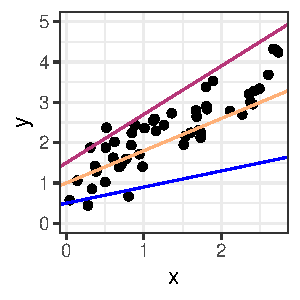
\includegraphics[width=\textwidth]{figure/reg_poly_linearity}
  \tiny \raggedleft
  \textcolor{blue}{$\thetab = (0.5, 0.4)^\top$} \\
  \textcolor{orange}{$\thetab = (1.0, 0.8)^\top$} \\
  \textcolor{magenta}{$\thetab = (1.5, 1.2)^\top$} \\
  \vspace{0.1cm}
\end{minipage}

\vfill

\item NB: we still call design matrix $\Xmat$, incorporating possible trafos:
\begin{align*}
  \Xmat =
  \left(
    \begin{smallmatrix}
        1 & \textcolor{black}{\phi_1} (x^{(1)}_1) & \ldots &
        \textcolor{black}{\phi_p} (x^{(1)}_p) \\
        % 1 & \textcolor{black}{\phi_2} (x^{(2)}_1) & \ldots &
        % \textcolor{black}{\phi_2} (x^{(2)}_p) \\
        \vdots & \vdots & & \vdots \\
        1 & \textcolor{black}{\phi_1} (x^{(n)}_1) & \ldots &
        \textcolor{black}{\phi_p} (x^{(n)}_p) \\
    \end{smallmatrix}
    \right)
\end{align*}
$\rightsquigarrow$ solution via normal equations as usual
\end{itemize}

\end{vbframe}

% ------------------------------------------------------------------------------

\begin{frame}{polynomial regression}

\begin{itemize}
    \item Simple \& flexible choice for basis funs: \textbf{$d$-polynomials}
    \item Idea: map $x_j$ to (weighted) sum of its monomials up to order
    $d \in \N$
    $$ \phi^{(d)}: \R \rightarrow \R, ~~
    x_j \mapsto \sum_{k = 1}^d \beta_k x_j^k$$
    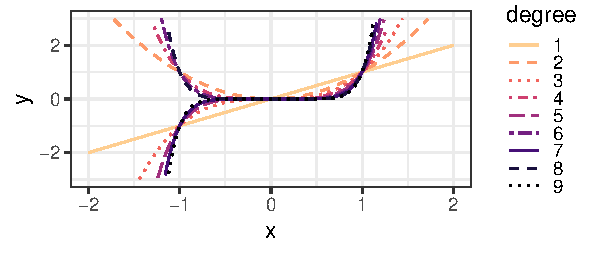
\includegraphics[width=0.9\textwidth]{figure/reg_poly_basis}
    \item How to estimate coefficients $\beta_k$?
    \begin{itemize}
      \item Both LM \& polynomials \textbf{linear} in their params
      $\rightsquigarrow$ merge
      \item E.g.,
      $\fx = \theta_0 + \theta_1 \phi^{(d)}(x)  =
      \theta_0 + \sum_{k = 1}^d \theta_{1, k} x^k$
      $$\rightsquigarrow \Xmat = \left(
      \begin{smallmatrix}
          1 & x^{(1)} & (x^{(1)})^2 & \hdots & (x^{(1)})^d \\
          \vdots & \vdots & \vdots & & \vdots \\
          1 & x^{(n)} & (x^{(n)})^2 & \hdots & (x^{(n)})^d \\
      \end{smallmatrix}
      \right),
      ~~ \thetab \in \R^{d + 1}
      $$
    \end{itemize}
\end{itemize}

\end{frame}

% ------------------------------------------------------------------------------

\begin{frame}{polynomial regression -- examples}

Univariate regression, $d \in \{1, 5\}$

\begin{minipage}[c]{0.5\textwidth}
  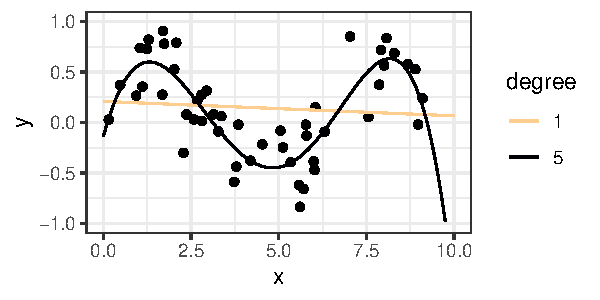
\includegraphics[width=\textwidth]{figure/reg_poly_univ_2}
\end{minipage}
\begin{minipage}[c]{0.45\textwidth}
  \begin{itemize}
    \footnotesize
    \item
    Data-generating process:
    \begin{align*}
      y &= 0.5 \sin(x) + \epsilon, \\
      \epsilon &\sim \normal(0, 0.3^2)
    \end{align*}
    \item Model: $$f(x) = \theta_0 + \sum_{k = 1}^d \theta_{1, k} x^k$$
  \end{itemize}
\end{minipage}

\vfill

Bivariate regression, $d = 7$

\begin{minipage}[b]{0.5\textwidth}
  \includegraphics[width=0.7\textwidth, trim=80 0 60 80, clip]{
  figure/reg_poly_biv}
\end{minipage}
\begin{minipage}[b]{0.45\textwidth}
  \begin{itemize}
    \footnotesize
    \item
    Data-generating process: 
    \begin{align*}
      y &= 1 + 2 x_1 + x_2^3 + \epsilon, \\
      \epsilon &\sim \normal(0, 0.5^2)
    \end{align*}
    \item Model: $$f(x) = \theta_0 + \theta_1 x_1 + 
    \sum_{k = 1}^7 \theta_{2, k} x_2^k$$
  \end{itemize}
\end{minipage}

\end{frame}

% ------------------------------------------------------------------------------

\begin{frame}{complexity of polynomials}

\begin{itemize}
  \item Higher $d$ allows to learn more complex functions 
  
  $\rightsquigarrow$ richer hyp space / higher \textbf{capacity}
  
  \vfill
  \includegraphics[width=0.8\textwidth]{figure/reg_poly_univ_4}
  \item Should we then simply let $d \rightarrow \infty$?
  \begin{itemize}
    \item \textbf{No}: data contains random \textbf{noise} -- not part of true
    DGP
    \item Model with overly high capacity learns all those spurious patterns
    $\rightsquigarrow$ poor generalization to new data
    \item Also, higher $d$ can lead to oscillation esp. at bounds 
    
    (Runge's phenomenon\footnote[frame]{\scriptsize
    Interpolation of $m$ equidistant points with $d$-polynomial only 
    well-conditioned for $d < 2 \sqrt{m}$. Plot: 50 points, models with $d \geq
    14$ instable (under equidistance assumption).
    })
    \vfill
  \end{itemize}
\end{itemize}

\end{frame}


% ------------------------------------------------------------------------------

\begin{frame}{bike rental example}

\begin{itemize}
    \footnotesize
    \item OpenML task \href{https://www.openml.org/search?type=data&sort=runs&id=45103&status=active}{
    \texttt{dailybike}}: predict \texttt{rentals} from weather conditions
    \item Hunch: non-linear effect of \texttt{temperature} $\rightsquigarrow$
    include with polynomial:
    \[
        \fx = \sum_{k=1}^d \theta_{\text{temperature}, k}
        x_{\text{temperature}}^k + \theta_{\text{season}} x_{\text{season}} +
        \theta_{\text{humidity}} x_{\text{humidity}}
    \]
    \item Test error\footnote[frame]{
    \scriptsize
    Reliable insights about model performance only via separate test
    dataset not used during training (here computed via 10-fold
    \textit{cross validation}). Much more on this in Evaluation chapter.
    } confirms suspicion $\rightsquigarrow$ minimal
    for $d = 3$
    \vfill
    \includegraphics[width=0.9\textwidth]{figure/reg_poly_bike}
    \tiny
    \begin{tabular}{rrrrrrrrrr}
        $d$ & $\theta_0$ & $\theta_{\text{temp}, 1}$ & $\theta_{\text{temp}, 2}$
        & $\theta_{\text{temp}, 3}$ & $\theta_{\text{sSPRING}}$ &
        $\theta_{\text{sSUMMER}}$ & $\theta_{\text{sFALL}}$ &
        $\theta_{\text{hum}}$ & \textbf{test error} \\ \hline
        1 & 377.3 & 2778.2 & & & 101.0 & 57.0 & 80.1 & -230.0 & \textbf{121.9}\\
        \rowcolor{black!10}
        3 & 419.3 & 2645.8 & -963.1 & -430.9 & 71.9 & 75.8 & 56.6 & -283.8 &
        \textbf{117.6}
    \end{tabular}
    \vfill
    \footnotesize
    \item Conclusion: flexible effects can improve fit/performance
\end{itemize}

\end{frame}



\endlecture

\end{document}
